\documentclass[12 pt]{article}
\usepackage[backend=biber, sorting=nyt, maxcitenames=2, doi=false,url=false, style=apa]{biblatex} %add annotation=true and style=reading to print the annotations in the bibliography
\usepackage[american]{babel}
%\usepackage{newtxtext,newtxmath}
\usepackage{csquotes}
\bibliography{input/all}
\DeclareLanguageMapping{american}{american-apa}
\usepackage[compact]{titlesec}
\usepackage{csquotes}
\usepackage{amsmath}
%\usepackage[hyphens]{url}
\usepackage[margin=1in]{geometry}
\setlength{\parskip}{.6em}
\usepackage{setspace}
\usepackage{multicol}
\usepackage{longtable}
%\usepackage{sectsty}
%\allsectionsfont{\singlespacing}
%\usepackage{indentfirst} %This indents the pfaragraph following a heading 
\usepackage[draft]{todonotes}
\newcommand{\smalltodo}[2][]
{\todo[caption={#2}, #1]
	{\begin{spacing}{0.5}#2\end{spacing}}}
\setlength{\parindent}{0em}
\usepackage{graphicx}
\graphicspath{{input/}} %make sure to include the slash after the colon at at the end 
%Make sure Bibliography --> is set as biblatex 
%Then run tools-->bibliography, then compile 

\title{\Huge Unifying theories of human action \\ \bigskip }
\author{\Large Harold Eyster, IRES PhD student}
\date{Comprehensive exam paper 2}
\begin{document}

	\maketitle
%	\fbox{\includegraphics[width=1 \textwidth,trim=0cm 0cm 0cm 0cm, clip=true]{comps_overview}}
\color {black}

\begin{abstract}
Sustainability scholars and practitioners have long relied on the natural sciences to understand environmental dynamics. However, to be successful, we must understand why humans -- a crucial driver of environmental dynamics --  do what they do. Unfortunately, these theories of why humans do what they do -- Theories of Human Action -- are strewn across multiple social science disciplines. This hinders interdisciplinary diffusion, preventing scholars from gleaning insights from other fields and developing a more unified theory of human action. To address this deficiency, I review and synthesize more than 50 Theories of Human Action from across the social sciences. I elucidate three metatheoretical underpinnings of these theories and reveal common action determinants. I end by adapting these metatheories and determinants into a unified framework. This framework, I hope, will spur a more interdisciplinary study of human action that enables sustainability scholars to finally understand why humans do what they do.   
\end{abstract}
\section{Sustainability needs social sciences}
Social sciences have historically played a small role in sustainability, though their importance  has long been explicitly recognized \parencite{Leopold1949}. Every sustainability issue has a human dimension, which social science is best positioned to address. Answering this call, the burgeoning conservation social sciences -- i.e., a subset of the classic and applied social science disciplines that focus particularly on conservation or environmental management -- are becoming more salient \parencite{Bennett2017,Teel2018}. However, the potential for social science transcends these fields that explicitly focus on the environment.  Copious social science research exists that is not pointedly conservation-focused, offering much to conservation. Whether coming from a study of energy use by psychologists \parencite{Schultz2007,Schultz2018} or diffusion of agricultural innovations by rural sociologists \parencite{Rogers2010,Mascia2018}, social science can provide much insight into sustainability. 

\subsection{Theories of Human Action are key for conservation}
What exactly makes these psychological and sociological studies useful? They are useful because they suggest why humans act the way they do -- i.e., they provide what I will call Human Action Theories.  Conservationists can take these findings about how humans act, and apply them to their own environmental systems of analysis. For example,  \textcite{Schultz2007} showed how human actions are in part determined by descriptive and injunctive social norms. This social norm theory of human action was then used by the company Openergy to persuade people to decrease their energy consumption. It worked. Over 10 years, utilizing social norm theory led to savings of more than  1 billion  dollars (USD) and 13 billion pounds of CO$_{\text{2}}$. This is the equivalent of the electricity needed to power 1 million U.S. homes for a year \parencite{Schultz2018}. 

Beyond actually changing human actions, \textit{Human Action Theories} can also offer many resources to researchers \parencite{Fawcett1978}. They can \textbf{organize, summarize}, and \textbf{communicate} research; explain what parts of the system should be \textbf{focused} on; and how to \textbf{observe} the focal aspects. Theories can \textbf{clarify} how to interpret these observations. When observations are sufficiently explained, theories can \textbf{guide} new research directions.  Perhaps  the most salient aspect of a theory may be its utility in \textbf{predicting} (modified from Bross, 1954; Littlejohn, 1983). In short, \textit{Human Action Theories} can aid sustainability scholars in identifying what factors are important for understanding, predicting, and affecting human action. 

\subsection{Problem: Human Action Theories are strewn across many disjunct fields}

However, there is no one human action theory to use.  Numerous human action theories are developed independently,  often in isolation, in many different social science fields and subfields. This independence makes using, comparing, and improving Human Action Theories difficult. Specifically, it prevents theory 1) \textbf{generalizability}, 2) \textbf{context internalizability}, 3) \textbf{complementarity}, and 4) \textbf{assumption explicability}.

 \subsubsection{Generalizability}
  For example, a social movement theory from Sociology, \textit{Polletta's Narrative Theory} and a theory of fulfilling action from educational psychology, \textit{Self-determination Theory} both stress the importance of autonomy: of not being externally directed \parencite{Polletta1998,Ryan2000,Ryan2000a}. Yet they call these factors different names: ``internal perceived locus of causality" (IPLOC) in \textit{Self-determination Theory} \parencite{Ryan2000,Ryan2000a} and ``spontaneity" in \textit{Narrative Theory}. This prevents cross-fertilization between these theories, and precludes any recognition of a generalized importance of this factor.  In short, the isolation of these theories prevents \textbf{generalizability}. 
 
 \subsubsection{Context internalizability} 
  Instead of sharing analogous factors, sometimes different theories have unique factors.  These differences could be important, in either revealing that one theory is missing something crucial (generalizability) or revealing key differences in theory contexts. For example, the \textit{Extended Parallel Process Model (EPPM)} does not contain an autonomy factor \parencite{Maloney2011}. Is this because, although autonomy is important, \textit{EPPM} scholars have simply not thought to examine it? Or is there something about the context under which \textit{EPPM} is applied -- fear appeals -- that makes autonomy not important? The dearth of interdisciplinarity prevents us from distinguishing between these options.  That is, differentiating between theory \textbf{generalizability} and \textbf{context internalizability} is prevented. 
  \textcite[][p. 172]{Bross1953} underscores the importance of explicit recognition of context-dependence: \blockquote{The evaluation of a model is therefore dependent on the situation in which it is used; it is not \textit{intrinsic} (i.e., dependent only on the model itself). If this point is understood several apparent paradoxes in science disappear. One such paradox is the simultaneous use of two contradictory models. An example of this paradox occurs in the field of physics in which a \textit{wave} and a \textit{photon model} for light are both accepted. Wave theories are used when \textit{they} provide successful prediction, and in other situations the photon theory is employed.}
  In other words, if the context and target of a model is not intrinsic to the model, then theory testing, building, and application will be hindered. 
  
 \subsubsection{Complementarity} 
Theory isolation also obfuscates complementarities between theories. These complementarities can provide synergies that improve each theory.  For example, although \textit{EPPM} does not contain an autonomy component, it does contain an effectiveness component, which is present in \textit{Self-determination Theory}. \textit{Self-determination Theory} posits that people feel ``competent" about something when they have self-efficacy \parencite{Ryan2000}. In contrast, \textit{EPPM} divides efficacy into two components: self-efficacy and response efficacy \parencite{Maloney2011}. Perhaps cross-pollinating \textit{EPPM} and \textit{Self-determination Theory} could make both theories stronger. Each theory may give a complementary assessment of the system \parencite{Weinberg2001}. Importantly, from the standpoint of a scientific observer, theories are constructions, representations, of human action. They are not a re-creation of the thing itself \parencite{Kaplan1964, Bourdieu1990}. Bourdieu (1990,  p. 12) writes: \blockquote{This construct, which the users would no doubt accept, and which makes it possible to account for the quasi-totality of the relevant facts (or those produced by observation or questioning armed with this model), or, rather, to recreate them, (theoretically) without being obliged to undertake an interminable narrative, is not as such the principle of agents' practice. The generative formula which enables one to reproduce the essential features of the practices treated as an \textit{opus operatum} is not the generative principle, of the process, the \textit{modus operandi.}}

In other words, theories are developed from a particular scholarly orientation, and reflect this orientation. They do not reflect the orientation of the human actor. Rather than trying to overcome this actor/observer or practice/abstraction  dichotomy, in this text I target the observer 1/observer 2/.../observer n   or abstraction 1/abstraction 2/.../abstraction n complexity, and attempt to understand the complementarities between them. In our example, a synergistic combination of these theories could perhaps advance both our understanding of how humans react to fear appeals, and how to intrinsically motivate them. 
\subsubsection{Assumption explicability}
Finally, different theories make different, and often implicit, assumptions about how humans act. Intertheoretical dialog can highlight these different assumptions, enabling us to contend with them directly. For example, \textit{EPPM} and \textit{Self-determination Theory} provide different strategies for explaining human action. \textit{Self-determination Theory} ``focuses primarily on psychological needs" \parencite[][p. 57]{Ryan2000}, while \textit{EPPM} is concerned with persuading people to make different choices. This reflects a fundamental and unanalyzed difference. Though both theories include an element of efficacy, EPPM looks to it as a driver of choice, while \textit{Self-determination Theory} examines it as a necessary condition for any meaningful action.  This results in different conclusions. For example, one might say that someone yells at a dog because the person perceived a loud noise,  while another might say it is because the person needed quiet. Highlighting these different approaches provides us with a more complete perspective of human action and demonstrates the importance of understanding how to use and compare different theories.

Overcoming these issues of generalizability, context internalizability, complementarity, and assumption explicability will create better theories that can facilitate sustainability. A unified framework of human action theories could be a key first step. 


\section{Unifying Human Action Theories}
This paper aims to create just such a unifying framework of \textit{Human Action Theories}. Other synthesis attempts have been made, but have been either directed at a narrower set of theories \parencite[e.g.,][]{Kollmuss2002}, \todo{if you're going to use e.g. here, you should also use it for Stern2018.. if not remove e.g.} or at practitioners \parencite{Stern2018}. \textcite{Kollmuss2002} explored diverse theories, but limited their analysis to pro-environmental behavior, i.e. behavior that \textit{consciously seeks} to better the environment. This is much narrower than my aim. Kollmuss and Agyeman (2002) also directed their findings only towards environmental educators. Again, I take a broader path, and hope that this will be useful to anyone thinking about the human dimensions of the environment.  Other scholars have looked specifically at decision theories in an energy context \parencite{Wilson2007}.  \textcite{Davis2015} attempted a full-spectrum review, but used search and analysis methods that prejudiced  non-psychology theories. One of the elements of their metatheory of theory utility was, ``clarity of constructs – `Has the case been made for the independence of constructs from each other?'" \parencite[][p. 332]{Davis2015}. This statement immediately prejudices theories of practice, where, ``in accounting for showering, the social, cultural and physical entities gathered under the labels of materiality, conventionality and temporality have no independent existence, none, that is, without the forms of `know-how', `competence', and `ways of doing' that represent and comprise what we currently understand showering to be." \parencite[][unpaginated]{Hand2005}. 
And ultimately, these reviews do not attempt to create a unifying framework \parencite{Davis2015}. Finally, others have directed their reviews at practitioners instead of scholars interested in interrogating and building theories:   \textcite{Stern2018} details how conservation practitioners can employ diverse theories, and begins to explain when and for what each theory is most appropriate. He provides succinct summaries of the theories, but he does not contend much with the theories themselves. 

Rather than repeating any of this work, I will contend directly with human action theories themselves (rather than how to employ them \textit{sensu} Stern (2018)), and will not limit myself to theories directed at conscious environmental behavior. My synthesis requires the following steps: 1) collecting a sufficient diversity of representative \textit{Human Action Theories}; 2) characterizing each theory's metatheoretical assumptions and action determinants; and 3) using these characterizations to construct a unifying framework. 
\subsection{Collecting representative Human Action Theories}
	\subsubsection{What are Human Action Theories?} 
	To gather theories from within the social sciences that attempt to describe the drivers of human action, a clear definition of Human Action Theory is required. I will use the following: \textbf{Human Action Theory:}  \textit{A description of a causative, directional relationship between a human action and a set of variables}. This definition differs from other conceptions of theory and human action. First, I conflate models, theories, and frameworks, \textit{sensu} \textcite{Littlejohn1983}, although there are distinctions \parencite{Hawes1975,Cox2016}. 
	
	Second, theory definitions often require that the causative variables are \textit{independent}. For example,  \textcite[][p. 47]{Cox2016} defines theories as describing, ``a relationship between an outcome and a set of independent variables...". However, this independence requirement excludes a dominant metatheoretical assumption in sociology and anthropology (see discussion about \textcite{Davis2015}, above). In the \textit{Theory of Practice}, action is a result of certain variables (habitus and fields), and simultaneously constitutes those same variables.
	
	Third, I intentionally use the term, `action' instead of `behavior.' Behavior is commonly used to refer to individual actions by fully agentic actors, and is centered in psychology  \parencite[e.g.,][]{Stern2000}. Indeed, much of the work on the human dimension of environmental issues has focused on individual `behavior,'  potentially limiting the body of knowledge accessible to environmental scholars \parencite{Shove2010}. Individual behavior theories form an especially dominant way of seeing the world -- environmental topologies -- both in research and policy arenas \parencite{Shove2010}. These topologies can exclude many relevant fields and other ways of analyzing problems and enacting solutions \parencite{Brosius1999}. Thus, I chose `action' as a term that has fewer disciplinary constraints. 
	\subsubsection{Selecting Human Action Theories}
	I do not seek to include every Human Action Theory, but instead a representative, diverse set. To collect theories, I employed a variety of methods: literature search,  cited sources,  and scholar consultation.  I conducted literature searches in Web of Science, using the following search terms ``(Social Science Field)" AND ``Theory" OR ``Model" OR ``Framework" AND ``Behavior" OR ``Action" OR ``Practice" OR ``Intention" OR ``Movement" OR ``Change,"  where social science field is the fields listed in Table \ref{tab:fields}.   I also found theories by following cited studies, and consulting with scholars from a diversity of fields, asking them about the dominant \textit{Human Action Theories} in their respective fields. Of these collected theories, I chose those for inclusion that were highly cited or representative. This left me with 54 theories (see Table \ref{tab:sources}). 
% latex table generated in R 3.4.0 by xtable 1.8-2 package
% Sun Nov 04 17:49:03 2018
\begin{longtable}{l|p{8cm}}
	\caption{Human Action Theories and selected sources} \label{tab:sources} \\
	\hline
	\textbf{Theory} & \textbf{Source} \\ 
	\hline
	Action and coping planning & \cite{Carraro2013} \\ 
	Attitude-behavior correlations & \cite{Kraus1995} \\ 
	Attitude, behavior, context  & \cite{Guagnano1995} \\ 
	Cognitive Dissonance  & \cite{Festinger1957,Festinger1959} \\ 
	Cognitive hierarchy of human behavior & \cite{Homer1988,Vaske1999} \\ 
	Collective action theory & \cite{Bimber2005} \\ 
	Cultural cognition of risk & \cite{Kahan2011,Kahan2012} \\ 
	Deficit model & \cite{Popkin1999,Sturgis2004} \\ 
	Deliberative democracy & \cite{Miller1992,John2009} \\ 
	Diffusion model & \cite{Oberschall1989} \\ 
	Diffusion of innovations & \cite{Rogers2010} \\ 
	Elaboration likelihood model of persuasion & \cite{Petty1986} \\ 
	Environment-behavior model & \cite{Hungerford1990} \\ 
	Environmental ethics & Reviewed in  \cite{Dickson2000} \\ 
	Environmentality & \cite{Agrawal2005} \\ 
	Environmental stewardship & \cite{Bennett2018} \\ 
	Environmental leaders  & \cite{Chawla2007} \\ 
	Exchange theory & \cite{Kotler2000} \\ 
	Extended parallel process model  & \cite{Maloney2011} \\ 
	Giradian economics  & \cite{Roe1996} \\ 
	Habits  & \cite{DeBruijn2007,Gardner2011} \\ 
	Health action process approach & \cite{Schwarzer2008} \\ 
	Health belief and preventative health & \cite{Rosenstock1974} \\ 
	Identity and agency in cultural worlds & \cite{Holland1998} \\ 
	Intentional norm change & \cite{Raymond2014} \\ 
	Model of ecological behavior & \cite{Fietkau1981} (summarized in \textcite{Kollmuss2002}) \\ 
	Motivation-hygiene theory & \cite{Herzberg1968} \\ 
	Motivation crowding--game theory  & \cite{Gneezy2000} \\ 
	Motivation crowding--norms & \cite{Gneezy2000} \\ 
	Narrative theory & \cite{Polletta1998} \\ 
	Norm activation model & \cite{Schwartz1977, DeGroot2009} \\ 
	Nudge theory & \cite{Wilk1999,Thaler2008} \\ 
	Psychometric paradigm  & \cite{Slovic1987} \\ 
	Reasonable person model & \cite{Kaplan2009} \\ 
	Relationship marketing & \cite{Morgan1994} \\ 
	Risk perception attitude framework & \cite{Rimal2001} \\ 
	Self-affirmation theory & \cite{Cohen2000} \\ 
	Self-determination theory  & \cite{Ryan2000, Ryan2000a} \\ 
	Self-efficacy & \cite{Bandura1977} \\ 
	Shared decision-making & \cite{Weiss1995} \\ 
	Social intuitionist model of moral reasoning & \cite{Haidt2001} \\ 
	Social movement framing & \cite{Benford2000} \\ 
	Social norms & \cite{Schultz2007, Farrow2017} \\ 
	Socioecological systems framework & \cite{Mcginnis2014} \\ 
	Stage model of fear communication  & \cite{DeHoog2007} \\ 
	Strength model of self-control  & \cite{Hagger2010} \\ 
	Systematic/heuristic processing & \cite{Chaiken1980} \\ 
	The Arithmetic of compassion & \cite{Vastfjall2016} \\ 
	Theory of planned behavior  & \cite{Ajzen1985} \\ 
	Thinking fast/slow & \cite{Kahneman2011} \\ 
	Transition management & Reviewed in \cite{Shove2007, Shove2010} \\ 
	Transtheoretical model of behavior change  & \cite{Prochaska1997} \\ 
	Value-belief-norm theory & \cite{Stern1999, Stern2000} \\ 
	\hline
	\hline
\end{longtable}
\section{Theory characterizations}
 Reaching back to the revolutionary work of Linnaeus, scientists have recognized that categorization is necessarily imperfect and sometimes arbitrary, but also very useful \todo{useful for what? maybe your next sentence should be a bit more explicit} \parencite{Dear2006}. My characterizations of \textit{Human Action Theories} are surely imperfect; despite this, I hope that they will advance our understanding of human action. 
\subsection{Disciplines represented}
\textit{Human Action Theories} are derived from a broad range of fields and subfields (see Table \ref{tab:fields}). Psychology, social psychology, and sociology provided a majority of the theories. Categorizations are based on where the theory was published, the identification of the authors, and the fields in which the theory was used. Not all theories fit cleanly into a field, preventing discreet \todo{or discrete?} categorization. In these cases, the theory was placed in the closest field, or in multiple fields. 

\todo{cap first letter of word on table}
\begin{center}
	\begin{table}
		\centering
		\caption {Number of theories used from each discipline} \label{tab:fields}  
		\begin{tabular}{|l | l|}
			\hline 
			\textbf{Field} & \textbf{Number of theories} \\
			\hline
			Environmental psychology & 2\\
			Health psychology/behavior & 4\\
			Educational psychology & 1 \\
			Psychology & 14 \\
			Social psychology & 9 \\
			Sociology & 9  \\	  
			Public health & 1 \\ 
			Economics & 6 \\
			Environmental ethics & 1 \\
			Marketing & 2 \\
			Anthropology & 4 \\
			Communications & 3 \\
			Political science & 3 \\
			Business & 1 \\
			Environmental education & 1 \\ 
			Education & 1 \\
			Science \& technology studies & 1 \\ 
			Interdisciplinary & 4 \\
			\hline
			\hline
		\end{tabular}
	\end{table}
\end{center}
\subsection{Cognitive assumptions: Thinking fast and slow }
Dual-processing has become an important way of understanding how humans treat information, especially in psychology and economics \parencite{Evans2008}. \textit{Dual-process Theory} suggests that there are two ways that humans process information, one is heuristic, unconscious, and fast; the other systematic, conscious, and slow \parencite{Chaiken1980,Evans2008,Kahneman2011}. This processing dichotomy goes back to Aristotle's \textit{Rhetoric}: he divides his persuasive appeals into two types: artistic (about the message itself) and inartistic (having to do with the context or attributes of the speaker)  \parencite{Aristotle1954,Littlejohn1983}. \textcite{Chaiken1980} shows how this content/context distinction is a result of dual-processing: content is salient under heuristic processing, while context dominates under systematic processing.

 Do most \textit{Human Action Theories} follow Aristotle's lead? Largely, no. Only a sixth of the theories contended with both cognitive processes. Nearly half were clearly directed at heuristic and/or systematic processing (though often implicitly) (see Figure \ref{fig:syst}). Of these 26 theories, most were directed solely at the systematic process. For the other theories, it remained ambiguous what sort of processing was required/targeted. This analysis reveals that many theories disregard the dichotomous way that we process information, potentially ignoring a key mediator of human action. I suggest that theorists be more explicit and intentional in their assumptions about how people process information.  
 
\begin{figure}
	\centering
	\textbf{Heuristic and systematic processing}  \medskip
	\fbox{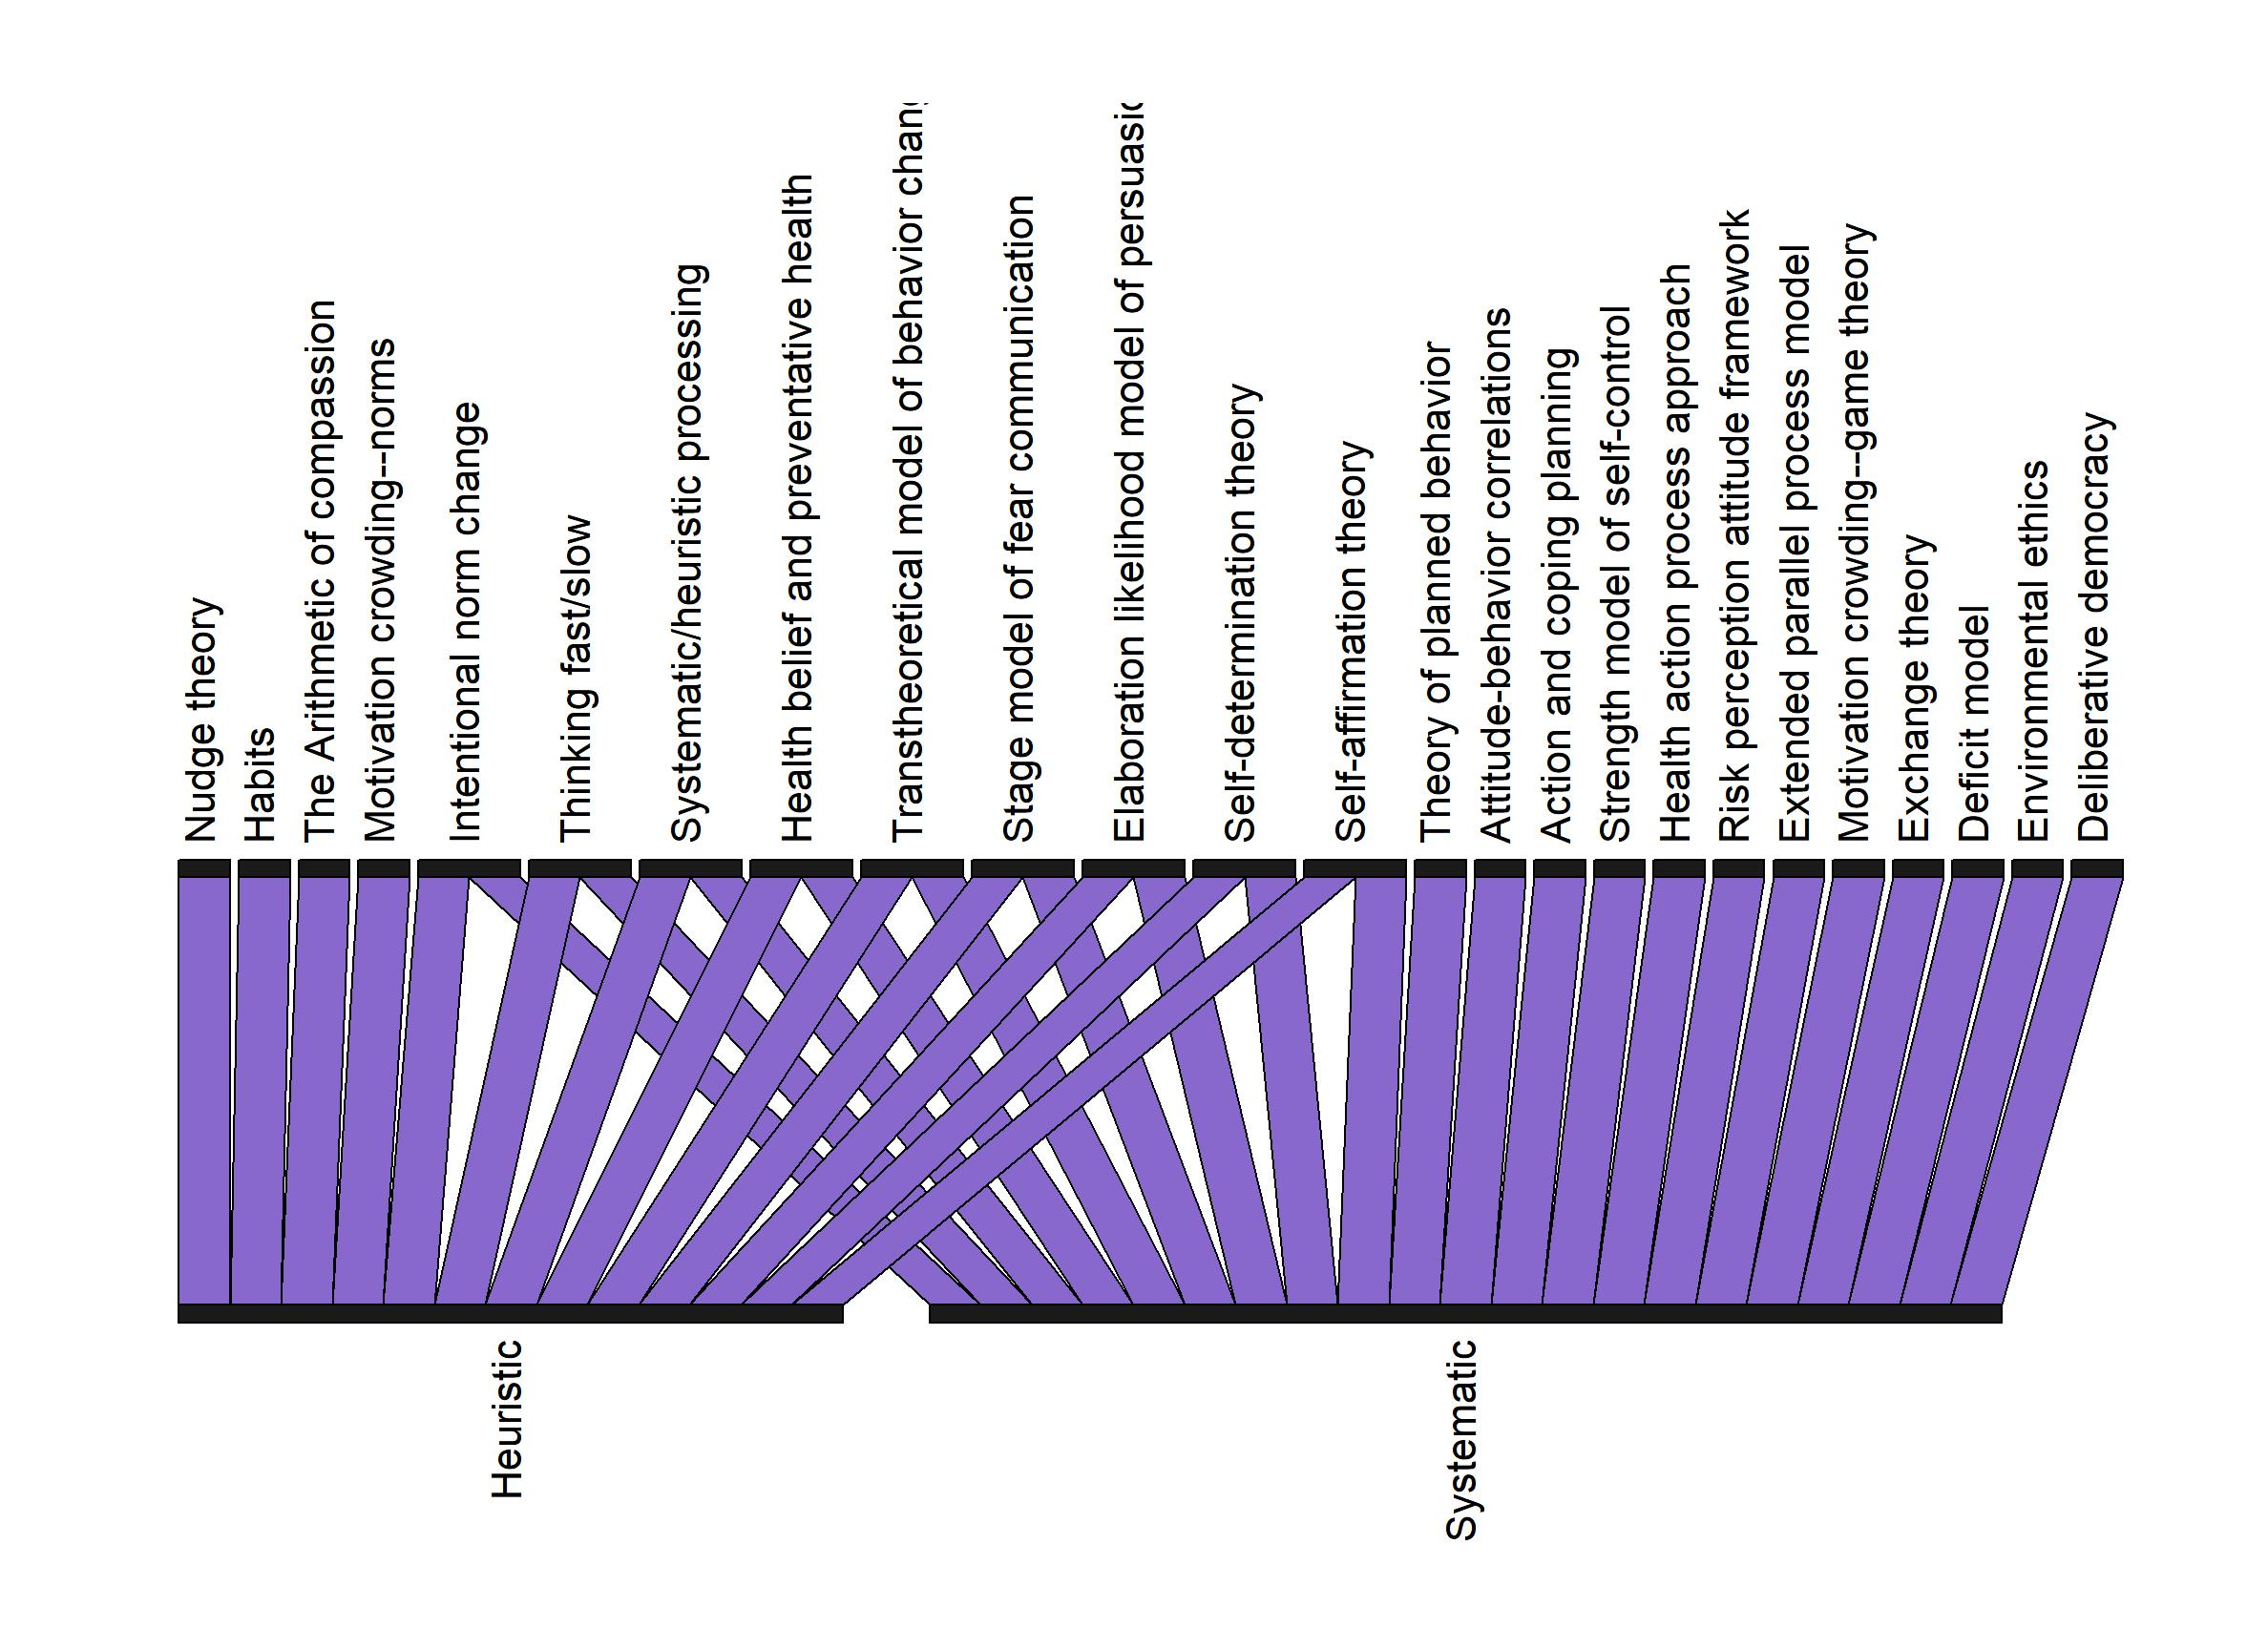
\includegraphics[width=1 \textwidth,trim=0cm 0cm 0cm 0cm, clip=true]{systematic}}
	\caption{\textit{Nearly half of theories -- 26 -- clearly treated humans as either operating using heuristic (i.e., thinking fast) and/or systematic (i.e., thinking slow) processing \parencite{Chaiken1980,Kahneman2011}. It was especially common for theories to employ just systematic processing, thus missing a bulk of the way that humans process the world. For the remaining theories, it was ambiguous which type of processing they were targeting.}}
	\label{fig:syst}
	
	
\end{figure}
\todo{FIG1: "The arithmetic of compassion" no caps on A}
\todo{FIG1: words are cut off on figure!}

\subsection{Metatheoretical assumptions of human action}
	 Metatheories tell researchers `...the sorts of questions one asks and
	does not ask...' \parencite[][p. 98]{Abrams2015}. These metatheories shape theories, though often implicitly \parencite{Fiedler2008}. This implicitness can frustrate efforts to harmonize divergent theories \parencite{Deci1976}. Explicating and relating these implicit metatheoretical assumptions can help to both 1) meaningfully compare different theories and 2) investigate each metatheory's  implication. 
	
	\textit{Human Action Theories} are steeped in metatheory. Metatheory tells human action researchers where to look for an explanation: ``If a human does X action, what Y could have caused it?" This limits the questions asked, and thus necessarily the answers obtained \parencite{Abrams2015}, and the implications of these answers. \textit{Human Action Theories} express three broad metatheory categories about why humans act the way they do, which I will call \textit{The Three I's: Interdependent, Independent, and Intrinsic} (see Figure \ref{fig:meta}). 
\begin{figure}
	\centering
	\textbf{Metatheoretical assumptions} \par \medskip
	\fbox{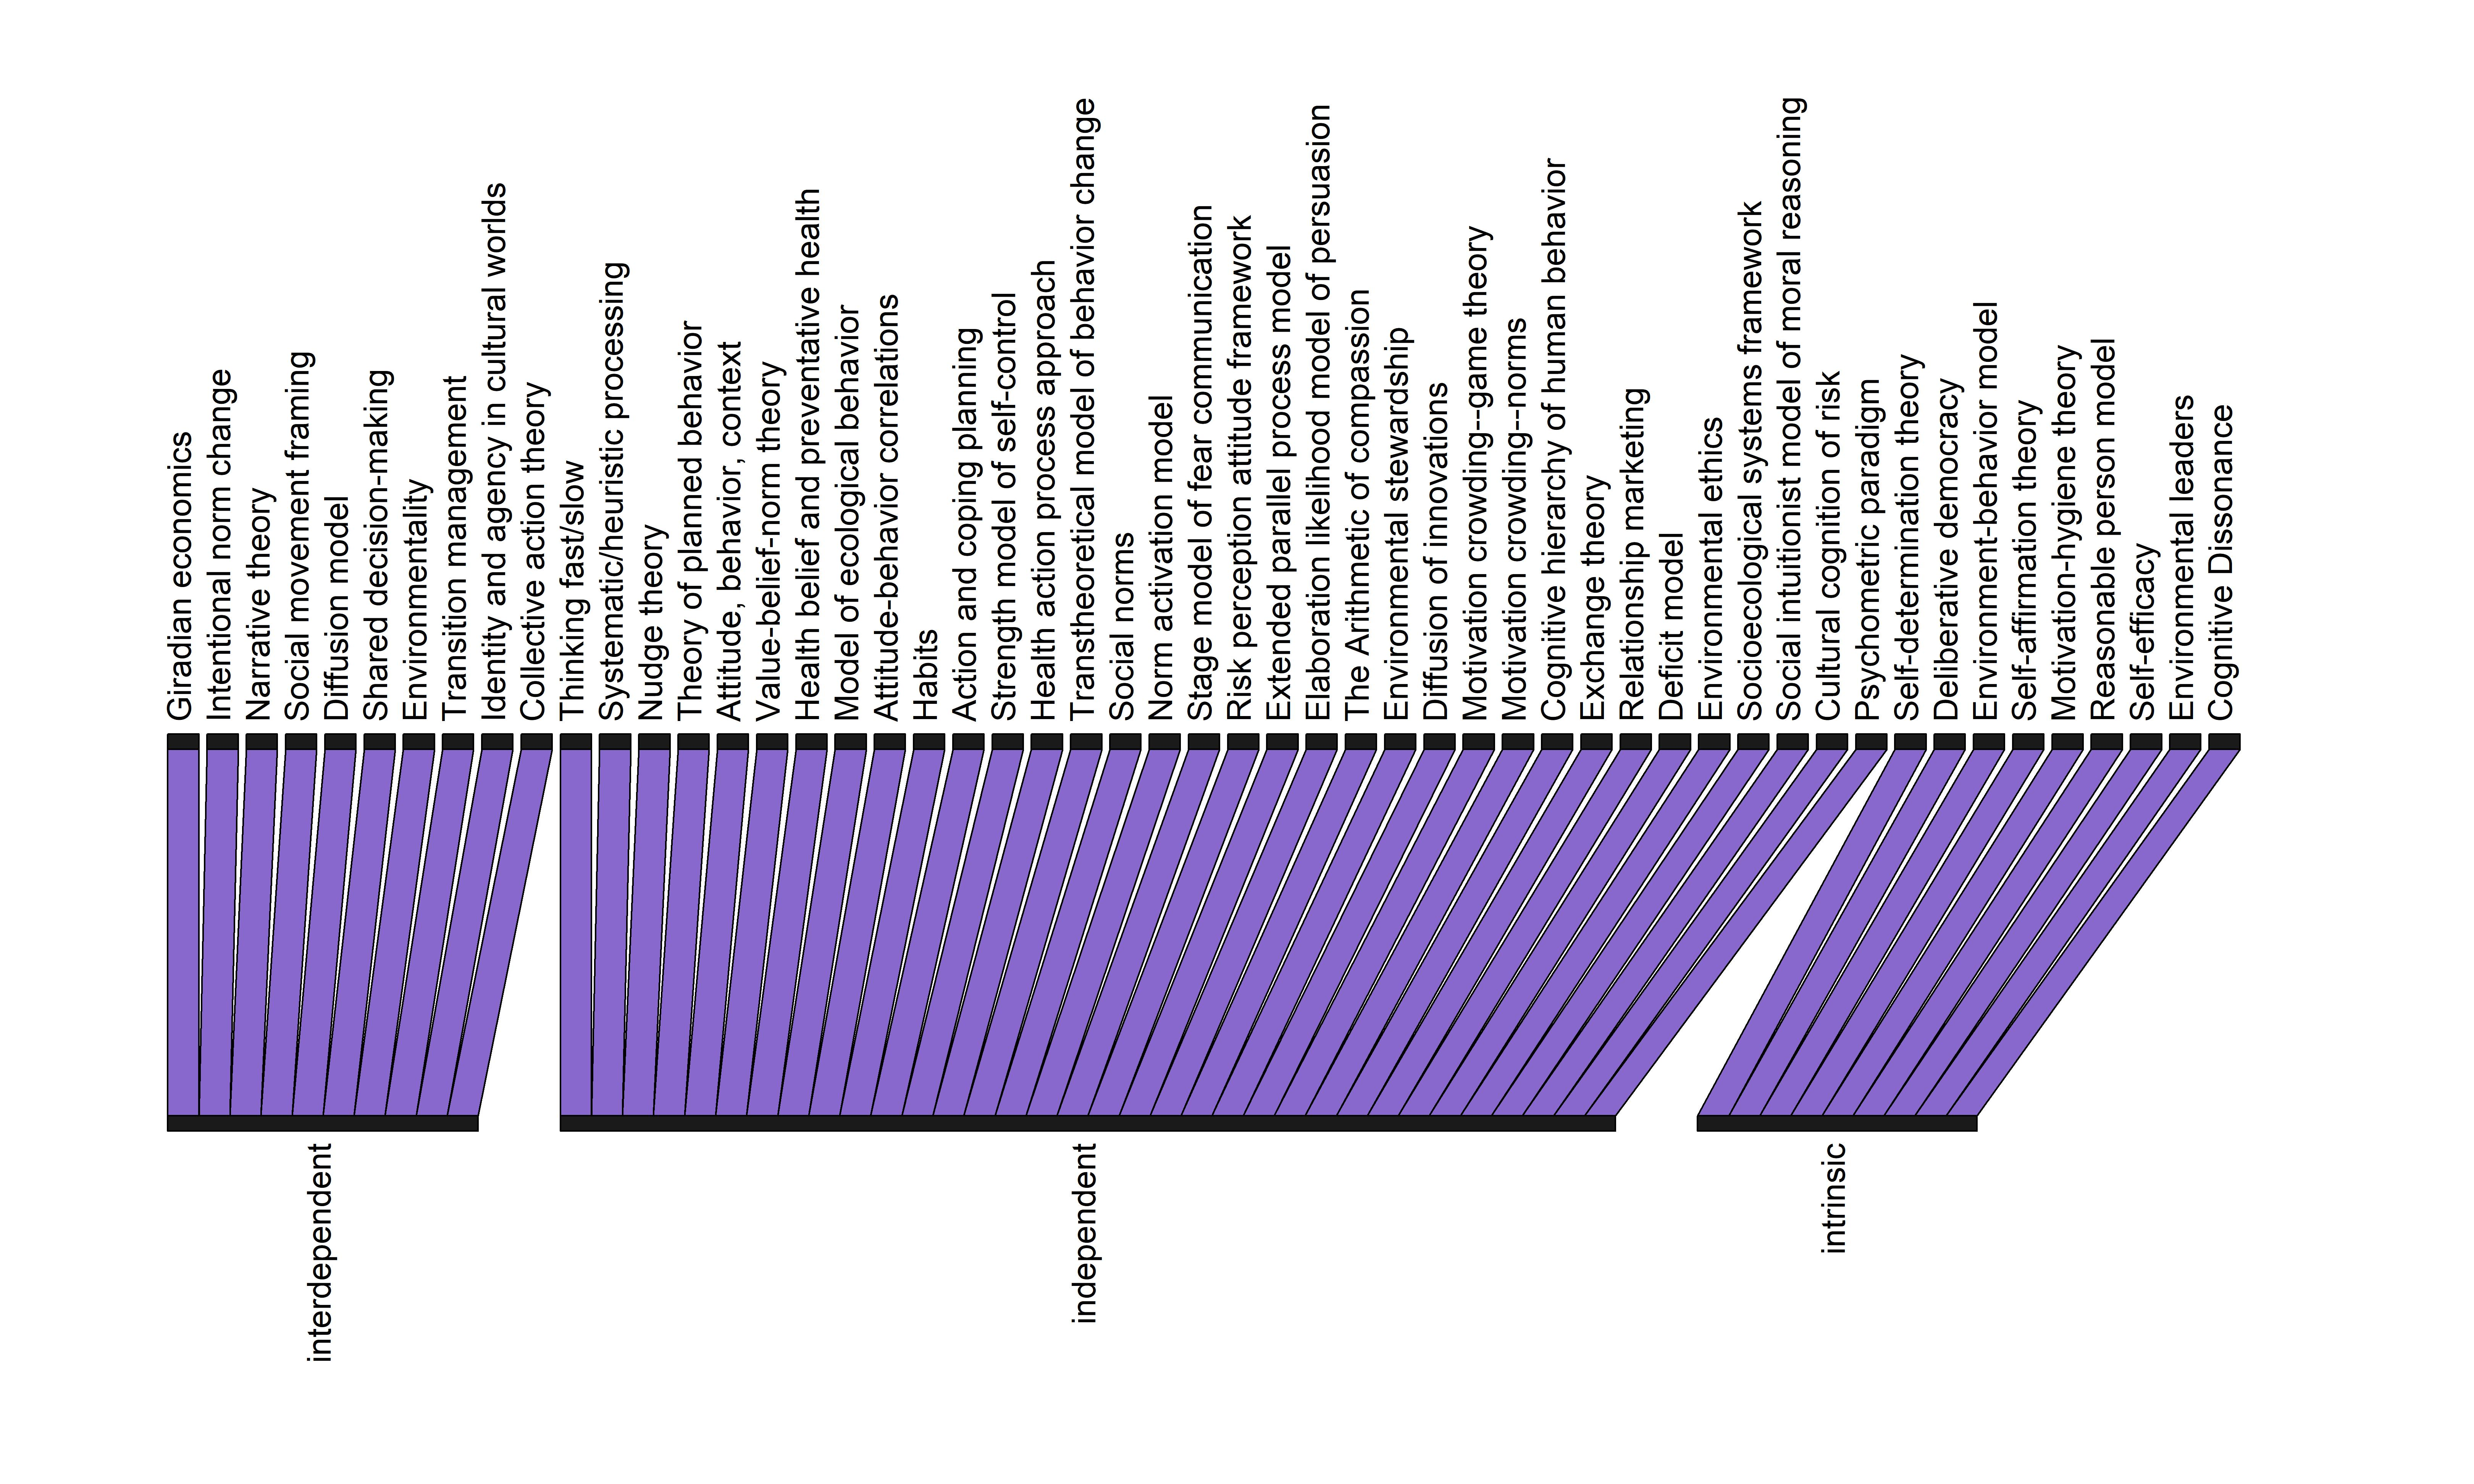
\includegraphics[width=1 \textwidth,trim=0cm 0cm 2cm 0cm, angle=270, scale=1.3, origin=c,clip=true]{meta}}
	%x x x lower right 
	\caption{\textit{Classification of the metatheoretical assumptions of each Human Action Theory.}}
	 \label{fig:meta}
\end{figure}	  
	\subsubsection{Interdependent} 
		This \textit{Interdependent Metatheory} sees human action as an emergent property of interdependent interactions between person and context.  A person's values, identities, habits, goals, needs, etc., are all dependent on the, e.g., institutions, cultures, and politics, and these same values, in turn construct these institutions. These variables then come together to constrain agency \parencite{Vigotsky1978} and lead to human action \parencite{Holland1998}. Action is both an \textit{output} and an \textit{input} in these theories.  These factors are unintelligible and nonexistent by themselves, indeed perhaps action is the only objectifiable attribute \parencite{Lewin1939,Bourdieu1977,Heft2012}. They must be considered in concert. Bourdieu's \textit{Practice Theory} is the archetype for much of the \textit{Interdependent Metatheory}, though I employ a less constrained version, allowing it to be an umbrella metatheory for a diverse set of theories. The key attribute of this metatheory is the co-developed interdependency of the constituent factors and the action. Thus, implying that no `way of life' can be taken for granted \parencite{Redclift1996}. Everything is malleable; it is impacted by and impacts everything else \parencite{Shove2010}.
		
		This metatheory has emerged from ten \textit{Human Action Theories} (see Figure \ref{fig:meta}), primarily coming from sociology and anthropology. For example, Dorothy Holland's \textit{Theory of Agency} (1998) and Arun Agrawal's \textit{Environmentality} (2005) both fit well within this metatheory. Although they use different terminology, both theories suggest that one's actions result from a codevelopment of the person, culture, and position. This is not to say that there is no agency, but that agency itself is also more or less constrained or enabled by these codeveloped factors. In \textit{Theory of Agency}, \textcite{Holland1998} states: ``This is our objective here: to respect humans as social and cultural creatures and therefore bounded, yet to recognize the processes whereby human collectives and individuals often move themselves  -- led by hope, desperation, or even playfulness, but certainly by no rational plan -- from one set of socially and cultural formed subjectivities to another."
		
		Sufficiently flexible spaces of authoring \parencite{Bakhtin1981} in combination with either 1) novel situations that create improvisation opportunities or 2) familiar situations and mediation tools \parencite{Vigotsky1978} enable agentic action \parencite{Holland1998}. This improvisational behavior is not merely the outcome of culture and situation, but also the beginning, an evolution, of new cultural forms. Improvisation occurs when past experiences, habitus, are brought to bear on novel situations \parencite{Bourdieu1977}. These improvisations are then in turn used as heuristics to ``guide, authorize, legitimate, and encourage" specific human actions \parencite[][p. 18]{Holland1998}. Thus, in the \textit{Interdependence Metatheory}, individual change is seen as an improvisation, not a choice. 
		
		Unlike other metathoeries which view factors as independent, the \textit{Interdependence Metatheory} focuses on that interaction. In \textit{Envrironmentality}, \textcite{Agrawal2005} writes about how the government's use of statistics to represent forests not only imperialized forests, it \textbf{made} forests. The conception of the trees cannot be extricated from the governance of them. 	
		
		Interdisciplinary theories also purvey this metatheory. For example, \textit{Transition Theory}: ``...it is important to remember that stakeholders' visions of the future are always and	inevitably shaped by the systems and social environments they inhabit today" \parencite[][p. 765]{Shove2007}. This demonstrates the interdependence between worldviews and `context'. Rather than viewing worldviews and values as static, this metatheory views these as dependent on everything else. This interdependence has strong implications for how we view change, for example, in using \textit{Transition Theory} to understand showering practice: ``change may occur as a result of disruptions within, and as a consequence of disjunctions between, the dimensions of materiality, conventionality and temporality, all of which are mediated by the practice itself" \parencite[][unpaginated]{Hand2005}. This metatheory posits that nothing can be taken  `as is'. That such things as conventionality and mateteriality are dynamic and worthy of analysis. Real, large-scale change requires that these things not be viewed simply as background context but as the ultimate causes of action. 
		
		This metatheory can be summarized as a response to the following parable:  ``it is as if trying to write the history of a marriage,
		one produces a biography of the wife, and placing it next to the biography
		of the husband calls it the history of the relationship itself!" (\textcite{White1995}, as paraphrased by \textcite[][p. 204]{Agrawal2005}). 
		
	
	\subsubsection{Independent}
	Under the \textit{Independent Metatheory}, action results from a meeting of the essentialized self and various proximate drivers. Each object can be understood in isolation, and context is poorly defined and  largely taken `as is'. The self does not affect the drivers or the context -- these are not interdependent. 

	
	For example, in contrast to theories embracing the \textit{Interdependent Metatheory}, \textit{Collective Action Frames Theory} takes the current world as it is, using `the culture out there' as an input \parencite{Benford2000}. This theory also includes `inherent ideology' as an important factor of determining a frame's resonance. As a mark of the metatheory, the self and culture are independent and static. However, theories do not always fit exactly into an idealized metatheory. Often while deploying the \textit{Independent Metatheory}, they make claims about their applicability for context-dynamic, interdependent worlds:  ``The lessons drawn from these studies are that changing cultural resonances and collective action frames reciprocally influence one another and that framing processes typically reflect wider cultural continuities and changes" \parencite[][p. 629]{Benford2000}. But something cannot be both inherent and mutable. This analysis highlights how implicit metatheories can lead to these internal inconsistencies. Making metatheories explicit will avoid these issues. \todo{rewrite last 3 sentences}
	
	\textit{Independent Metatheory} dominates \textit{Human Action Theories} -- shaping 35 of these theories (see Figure \ref{fig:meta}). This metatheory is similar to Shove's (2010) category of \textit{`ABC' (Attitude, Behavior, Choice)} theories. Shove demonstrates the power of this pervasive metatheory in science and policy: when presented with unexplained human action, ``the tendency is to commission further studies in the same mold. This results in a self-sustaining paradigm" (2010, p. 1276). This cyclical relationship with policymakers is a self-reinforcing barrier to innovative thinking (like a stagnant Community of Practice \parencite{Wenger1998}). 
	
	How does change happen in the \textit{Independent Metatheory}? While change under the \textit{Interdependent Metatheory} occurs by changing the ultimate, underlying societal factors themselves, \textit{Independent Metatheory} sees change as happening by rearranging proximate stimuli or reshaping values. Additionally, while \textit{Interdependent Metatheory} takes a large-scale and dynamic view of the world, \textit{Independent Metatheory} perspectives are most relevant at the terminus of the co-developed social, cultural, and subjective (\textcite{Uzzell2008}, as cited by \textcite{Shove2010}). 

	\subsubsection{Intrinsic}
	The third and final metatheory views human actions as driven by intrinsic needs. This theory has the smallest representation among my \textit{Human Action Theories}, with nine theories operating under the \textit{Intrinsic Metatheory} (see Figure \ref{fig:meta}). For example, \textit{Self-determination Theory} \parencite[][p. 132-3]{Deci1976}:  \blockquote{...[A]ssumes that people choose what to
		do in order to achieve their desired end-states. That is not to say that
		people have free will nor even that all the decision-making is conscious;
		it is only to say that behavior is understandable and predictable and that
		a decision-making framework that views people as working to attain goals having psychological value to them seems to be a productive way of studying behavior.} 
	 Unlike the other metatheories, \textit{Intrinsic Metatheory} starts with the person. It first asks the question, ``What are the needs" and then the world is analyzed in the context of these needs. The factors that seem relevant to these needs become the possible drivers of behavior. This metatheory is more human-focused than the preceding two -- it only examines external drivers after deciphering the human needs. These \todo{which theories?} theories are agnostic as to whether behavior and the attributional factors are interdependent or not, however, the foundational human needs \textit{are} independent and universal. For example, \textit{Cognitive Dissonance Theory} has been used to show that behavior affects attitudes, but the underlying needs for conquering cognitive dissonance are assumed to remain impervious \parencite{Festinger1959}. It further assumes that needs are culturally and socially conserved. 
	 
	 \textit{Intrinsic Metatheory} often has a strong well-being motivation: if conditions are created that enable humans to meet their needs, then human well-being will improve. For example, \textit{Self-determination Theory} shows how to meet human needs for autonomy, which in turn cultivates well-being \parencite{Ryan2000a}.
	 
	 While the \textit{Independent} and \textit{Interdependent Metatheories} tell us what assumptions to make about the interactions between different factors, the \textit{Intrinsic Metatheory} tells us to focus on the internal needs, and are often motivated by larger normative goals such as wellbeing, reasonableness, or environmental responsibility \parencite{Hungerford1990, Ryan2000a,Kaplan2009}.
	 
	 	\subsubsection{Reconciling the Three I's}  The \textit{Three I's of Human Action Theory: Interdependent, Independent, and Intrinsic},  represent idealized assumptions about how to understand human action. Some argue that these differences make them incommensurable -- going so far as to even call the \textit{Independent Metatheories} `useless' \parencite[][p. 1202]{Shove2010} I doubt this is so. While these metatheories reflect significant differences in perspectives about how the world works, I posit that people of all ideologies can see the usefulness of different metatheories in different contexts. 
	 	
	 	 When conservationists are interested in local and limited individual changes, the \textit{Independent Metatheory} may be most effective. These theories take everything else as given, and are able to focus on what proximal variables can most easily be changed \parencite{Hastings2003}. On the contrary, if trying to mitigate the global, transocietal problem of climate change, \textit{Interdependent Metatheory} may be best suited \parencite{Shove2010}. They can view everything as changeable, which may be necessary to bring about the huge changes that global warming requires. Finally, to make these changes sustainable, human needs may need to be accounted for, making the \textit{Intrinsic Metatheory} appropriate \parencite{Herzberg1968,Ryan2000a}. Each of these metatheories are best suited to tackle different problems. Directly analyzing the metatheory underpinning each theory enables researchers and policymakers to understand and implement the best solutions for every problem. 
	 
\section{Determinants of Human Action}
While the metatheories underpinning each theory are often implicit, the factors that each theory uses to determine human action are explicit and easily gathered. These determinants present what theory elements are important. I collected determinants from all selected theories and categorized them into 24 emergent classes (see Figure \ref{fig:fact}).  As outlined earlier with respect to autonomy, different theories use different names for similar determinants. This can make uniting them difficult, but I attempt to do this with my categorizations. Figure \ref{fig:fact} shows the relationships between theories and their determinants, facilitating comparison. Some determinant classes reach across many theories (e.g., response efficacy), while others are confined to a handful of theories (e.g., exploration). Relating each theory's determinants enables us to easily compare them and identify potential generalities, complementarities, and context-specificities. Below, I outline the role of each determinant class.
\begin{figure}
	\centering
	\textbf{Determinants used in Human Action Theories}\par \medskip
	
	\fbox{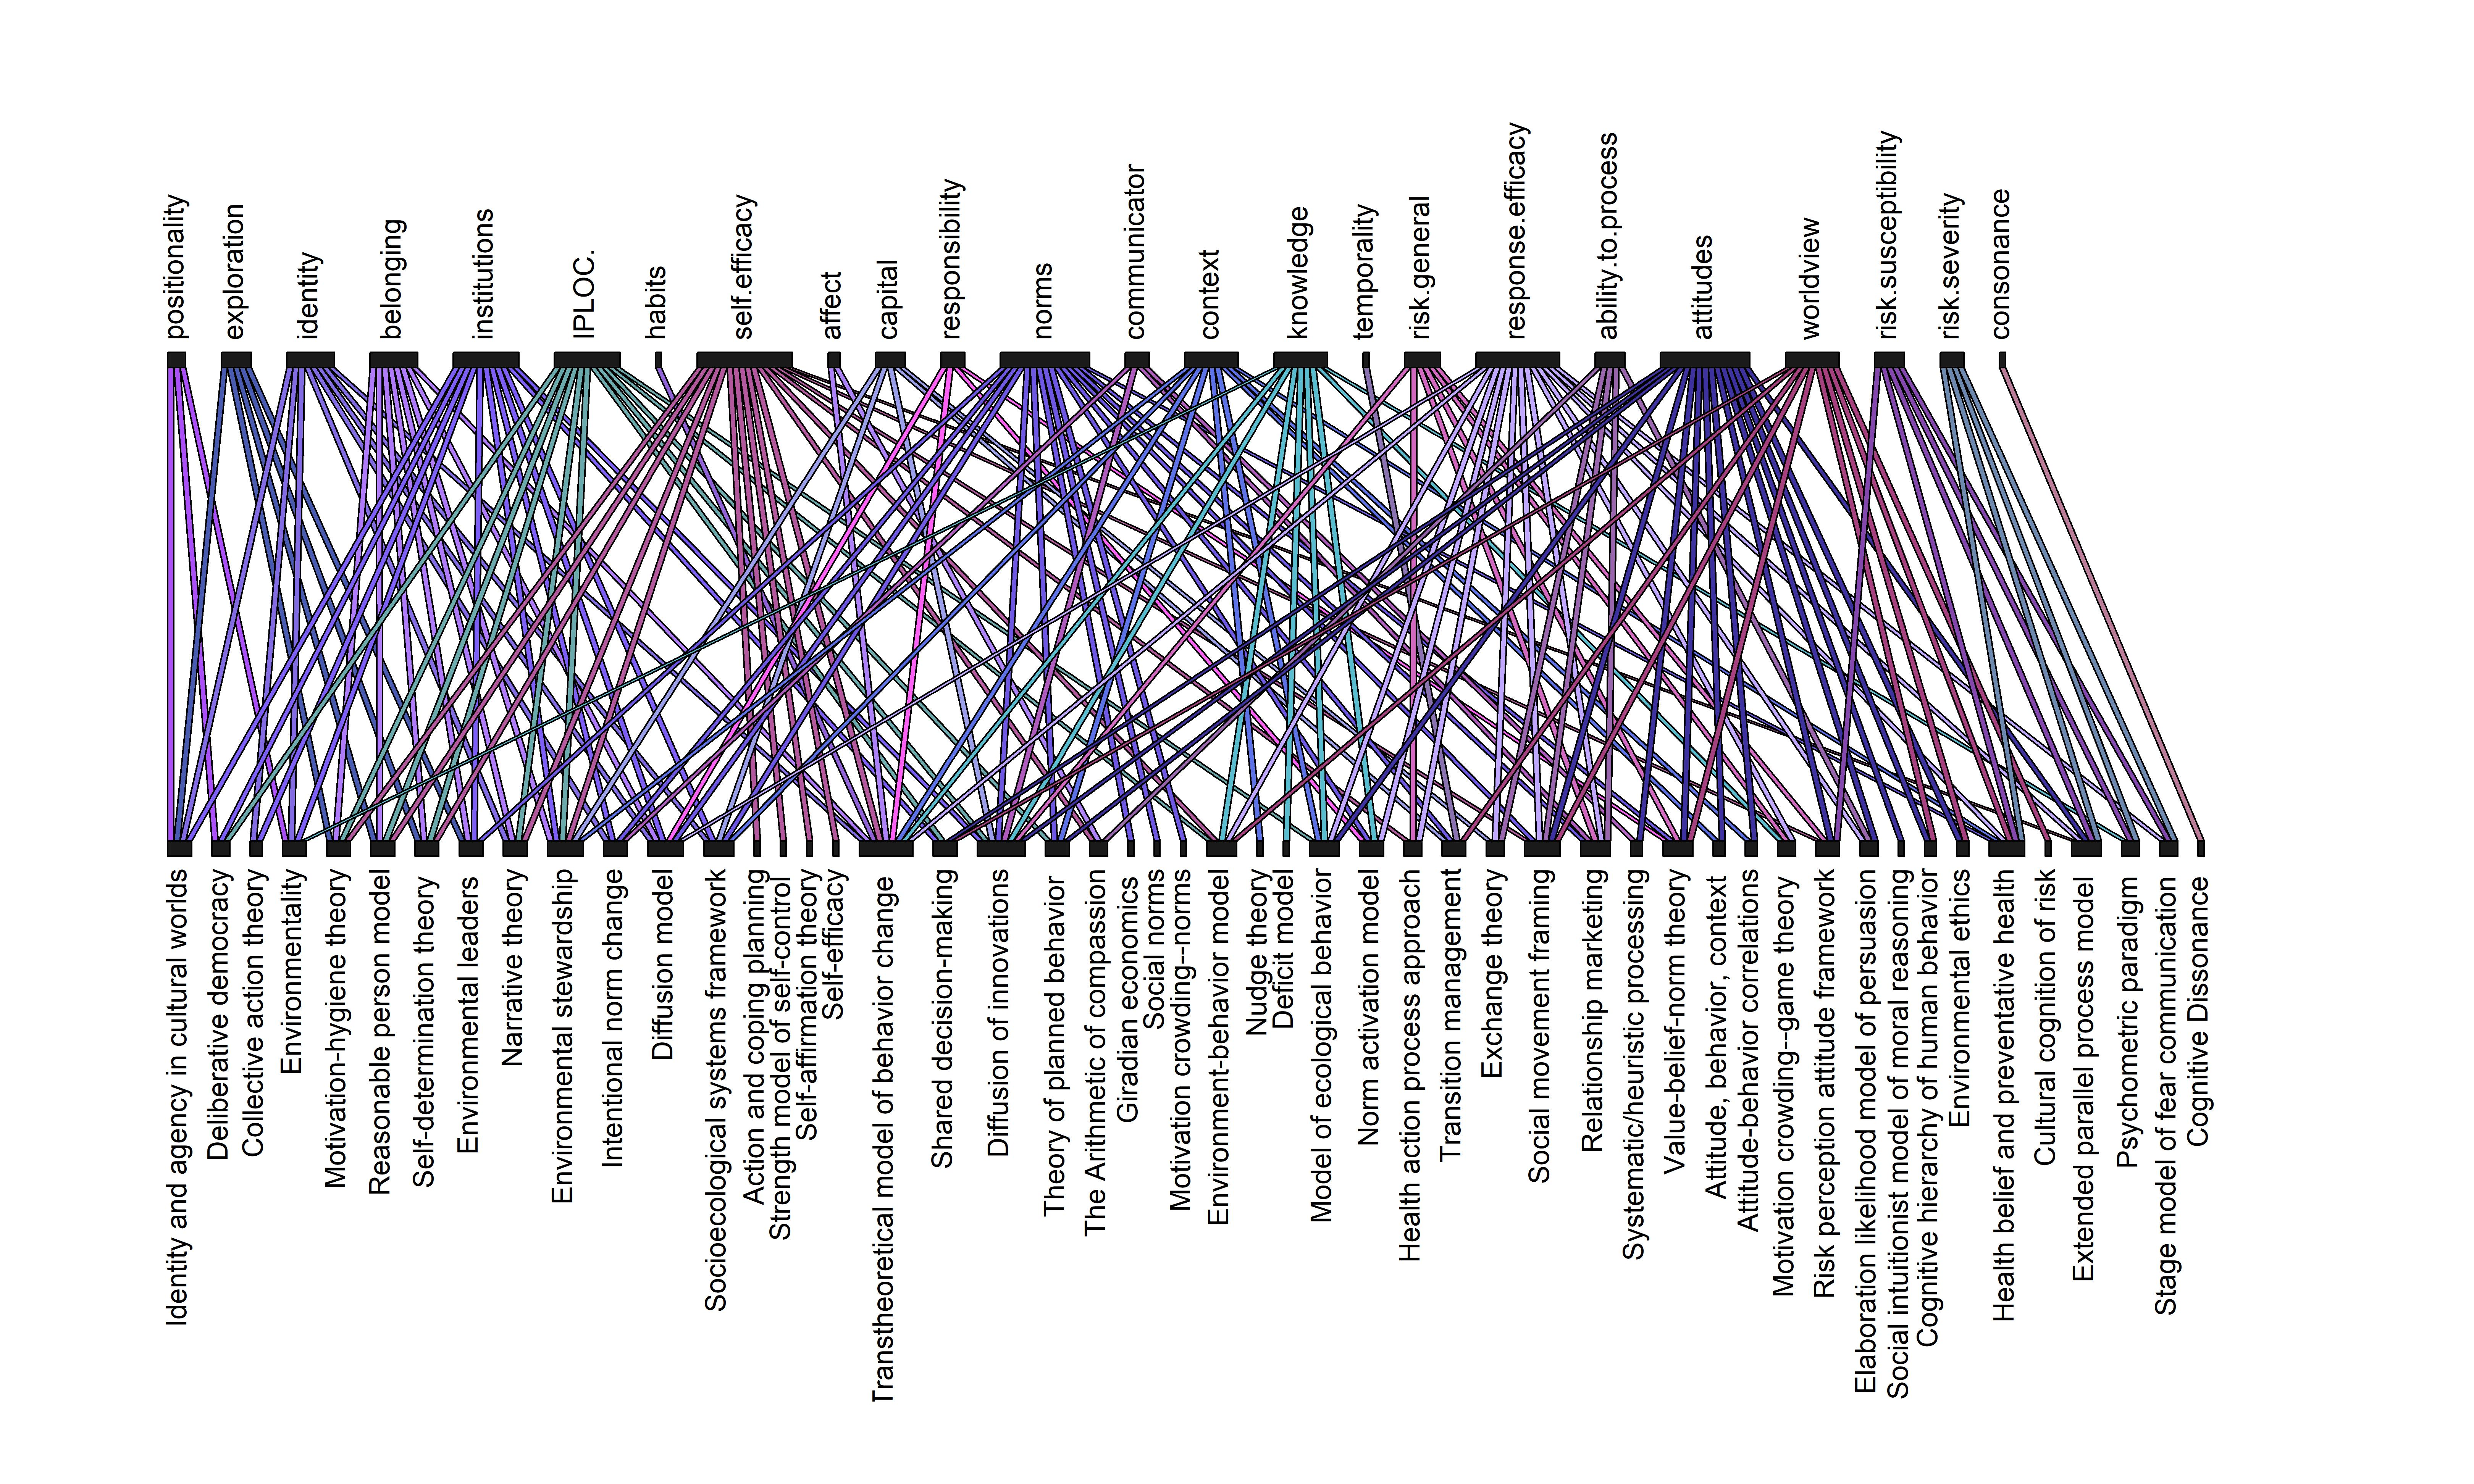
\includegraphics[width=1 \textwidth,trim=2cm 0cm 4cm 0cm, angle=270, scale=1.3, origin=c,clip=true]{fact}}
	%x x x lower right 
	\caption{\textit{Each theory is listed on the left, and each of the emergent determinants is on the left. A connection demonstrate that a theory encodes a given determinant. Note that this plot merely shows what determinants each theory encodes -- it does not show the relationships between determinants, nor the way in which they affect action (or vice versa)}}
	\label{fig:fact}
\end{figure}
		\subsection{Identity}
		`Identity' comes largely from anthropology and sociology. Identity is the subjectivity of Agrawal's \textit{Environmentality} (2005) and identity of Holland's (1998) figured worlds \todo{is this a title? if so \textit{}}.  Unlike culture, which is assumed to be everywhere, figured worlds are socially produced, culturally  constructed activities \parencite{Holland1998}. Figured worlds create identities, and turn landscapes into peopled \todo{is this a word?} experiences, replete with rich histories and stories.  
		
			
		In line with the \textit{Interdependence Metatheory}, identity is often seen as dynamic and as a process, not a state. According to \parencite{Holland1998}, identity is the sociogenic ``imaginings of self in worlds of action" (p. 5). Identities shape what we care about, and how \todo{how what?}. Anthropological conceptions of identity often focus on ethnicity, gender, and race. \textcite{Holland1998} instead conceptualizes identity as developing through practices within ``socially enacted, culturally constructed" worlds (p. 7) and aims to ``build upon and move beyond two central approaches -- the culturalist and constructivist -- to understand people's actions and possibilities. ``All the perspectives we discuss assume, at least implicitly, that behavior is mediated by senses of self, or what we call identities." (p. 8).  Some identities may be more omnipresent, e.g., gender, but is still differently strong in different contexts, and are not essentialized \parencite{Agarwal1992}.
	
		\subsection{Worldview}
		Worldview bears similarities to identity, but often comes from psychology and social psychology. This determinant class combines values, beliefs, etc., and I define it as trans-situational, long-standing beliefs about the world. \textcite{Kahan2011} harnesses worldviews about social organization to understand risk perception in his \textit{Cultural Cognition of Risk Theory}. Stern (1999, 2000) uses the \textit{New Ecological Paradig} to measure beliefs about the environment, which are then used to predict pro-environmental behavior.  Worldviews, unlike identities, are often heavily quantified.  
		\subsection{Attitudes}
		While worldviews are seen as target-transcendent, attitudes are normally directed towards an object \parencite{Hitlin2004}.  Attitudes are nearly omnipresent in the psychological theories of human action (see Figure \ref{fig:fact}). These theories hold attitudes as being all-important in leading to action \parencite{Kraus1995}, though others struggle to find such a clear relationship \parencite{Sniehotta2014}. 
		\subsection{Affect}
		 While attitudes are somewhat stable, affect is temporary and can be nebulous. \textcite{Vastfjall2016} suggests that there are two types of affect: incidental (exogenous; independent of the signal) and integral (endogenous; derived from the signal) \parencite{Loewenstein2002}. In an early experiment, \textcite{Johnson1983} showed the importance of this incidental affect. These two factors are consistent with Lewin's \textit{Field Theory} -- i.e., that the response to a target is a result of the interaction between the target and the person's experiences \parencite{Lewin1939}. Thus, as \textcite{Johnson1983} found, the experience of reading a newspaper will affect your response to your future environment. Thus, through all of this, we see the importance of 1) the object itself and 2) the incidental affect of the subject (as determined by previous experiences). 
		
		Affect pulls from a number of theories, primarily in psychology. For example \parencite{Prochaska1997} notes the importance of dramatic relief -- `increased emotional experience' -- for changing addictive health behavior. \textcite{Prochaska1997} are referring to integral affect. \textit{Human Action Theories} typically examine integral affect, not incidental.  However, different scholars define affect, emotion, and moods, etc., differently. This makes disentangling them difficult. Incidental emotions (directed at a specific target) may be transferred towards new, unrelated targets \parencite{Loewenstein2002}, affecting things like the endowment effect \parencite{Lerner2004}. However, because the cause of emotions is more salient, incidental emotions may impact decisions less than incidental moods \parencite{Vastfjall2016}.  This effect of incidental affect on, e.g., altruistic action can be reduced by pointing out that the mood is caused by extraneous factors \parencite{Schwarz1983,Schwarz2012}. 
		\subsection{Habits}
		Psychology theorists use habits to attempt to account for, and close, the intention behavior gap \parencite{DeBruijn2007,Gardner2011}. Though, as Shove (2010) has noted, using behavior to predict behavior seems a bit circular. 
		\subsection{Norms}
		Norms provide rules that, often unknowingly, govern the ways we act \parencite{Raymond2014}. Norms are widely used (see Figure \ref{fig:fact}).  Those within the \textit{Interdependent Metatheory} see norms as changeable and that every human action sustains or upturns these norms \parencite[e.g.,][]{Raymond2014}. \textit{Independent Metatheory}, on the other hand, often view norms as a fixed part of the `world out there' that affects behavior and can be harnessed to change behavior in desirable ways \parencite[e.g.,][]{Ajzen1985,Schultz2007}. 
		\subsection{Capital}	
		Capital corresponds to the reservoirs that actors can draw upon. It is diverse, including natural resources -- physical capital -- in Ostrom's \textit{Socioecological Systems Framework} \parencite{Mcginnis2014}, or social and other forms of capital in Bennett's \textit{Environmental Stewardship Framework} \parencite{Bennett2018}, or marketable goods and services in \textit{Exchange Theory} \parencite{Kotler2000}. 
		\subsection{Temporality}
		Temporality speaks to the ordering and sequencing of (often recurring) events \parencite{Hand2005}. Temporality is found in \textit{Interdependent Metatheory}, and is not widely used. 
		\subsection{Institutions}
		This class represents a diverse set of determinants, and is heavily relied upon in \textit{Human Action Theories}, especially those coming from sociology and anthropology. Institutions represent the merging of the state and society in Agrawal's (2005) \textit{Environmentality}, and \textit{Culture} for Holland (1998). Institutions are the social systems that constrain diffusion in Roger's \textit{Diffusion of Innovations Theory} (2010), and purvey norms in Raymond's \textit{Intentional Norma Change} (2014). \todo{sometimes you put the year before the theory and sometimes after. Be consistent.}
		\subsection{Positionality}
		Positionality is the instantaneous social and environmental position that people find themselves in. It draws from constructivism \parencite{Holland1998}, and encodes factors like rank, power, etc. Positionality is identified as `politics' in Agrawal's \textit{Environmentality} (2005). Many theories ignore these factors or dismiss them as `context' \parencite{Shove2010}. 
		\subsection{Context}
		 Theorists (especially those assuming on \textit{Independent Metatheory)} often identify context as an annoyance that clouds their controls  \parencite{Ajzen1985,Shove2010}, or as a variable to make small, easy, changes in order to affect unconscious behavior (e.g., nudges \parencite{Thaler2013}. Because context is hard to measure, theorists are often loath to include it in an operational way. Many have suggested that people are more sensitive to context when using heuristic processing (i.e., thinking fast) \parencite{Chaiken1980,Thaler2008,Kahneman2011}. 
		\subsection{Communicator}
		Who is the communicator? Rather than the message, sometimes the context of the communicator -- i.e., who they are -- is important for determining action \parencite{Chaiken1980}. For example, in \textit{Diffusion of Innovations Theory}, communicators who are more similar to their audience more successfully diffuse novel practices \parencite{Rogers2010}. 
		\subsection{Risk (general)}
		Risk is the degree of threat from something. Unlike norms, outlined above, risk represents a different philosophical understanding of the world. Norms tell us how to act (deontological), whereas risks tell us something about the results of our behavior (consequentialist). Risk perception is a staple of many theories, especially those coming from health psychology (e.g., Rosenstock, 1974). However, risk is not limited to psychology: it's also a central component of sociological social movement theories. For example, in \textit{Collective Action Frame Theory},  \textcite{McAdam1996} notes that successful social movements frames must combine aggrievement and optimism, where we can construe aggrievement as risk and optimism as efficacy. Some theories -- e.g., \textit{Risk Perception Attitude Framework}, -- hold that there is an interaction between risk and efficacy \parencite{Rimal2001}, while others -- e.g., the \textit{Stage Model of Fear Processing} \parencite{DeHoog2007} -- assume there is not. Like McAdam, some theorists use a general conception of risk; others break risk into two constituent parts: risk severity and risk susceptibility \parencite{Maloney2011}. 
		\subsection{Risk severity}
		Risk severity is the magnitude of the risk -- e.g., will an asteroid wipe out all of humanity, or will one person get a mild fever? Sometimes only one of type of risk -- risk severity or risk susceptibility -- is used \parencite[e.g.,][]{Rimal2001}. However, other theories have demonstrated that risk severity and risk susceptibility have different and interdependent effects \parencite{DeHoog2007}.
		\subsection{Risk susceptibility}
		Risk susceptibility also known as vulnerability, is the likelihood of a risk actually occurring. This is more commonly measured than risk severity (see Figure \ref{fig:fact}). Beliefs about risk susceptibility also depend on the type of processing being used (heuristic vs. systematic). 
		\subsection{Knowledge}
		Knowledge is seen by many non-social scientists as the leading cause of inaction or wrong action. This is the \textit{Deficit Model} of human action. If people only had more knowledge they would act. Although this simple linearity is not supported \parencite{Sturgis2004}, information is still included in many theories. \textit{Environmentality} notes how statistical knowledge redefines the way villagers treat nearby forests \parencite{Agrawal2005}, and the \textit{Transtheoretic Model of Behavior Change} includes knowledge of healthier behaviors as a key attribute. 
		\subsection{Response efficacy}
		Response efficacy reflects the belief that one's actions will have a desired result. This and self-efficacy are two of the most widely used determinants (see Figure \ref{fig:fact}). Some theories include both this and self-efficacy \parencite[e.g., \textit{EPPM} --][]{Maloney2011}, while others include only self-efficacy \parencite[e.g.,][]{Rimal2001}, while still others only include response efficacy \parencite[e.g.,][]{DeHoog2007}.    
		
		\subsection{Self-efficacy}
		Self-efficacy reflects the belief that one can carry out a desired action. This determinant includes maintenance and recovery of self-efficacy \parencite{Schwarzer2008}, self-control \parencite{Hagger2010}, competence \parencite{Ryan2000}, and coping \parencite{Carraro2013}. The dominance of efficacy among these theories make it seem like a generalizable determinant of human action. 
		
		\subsection{Ability to process}
		Ability to process encodes the ability to comprehend a problem and understand a message. It is used to understand how someone  interprets a social action frame \parencite{Benford2000}, and messages about unpleasant things \parencite{Vastfjall2016}. 
		
		\subsection{IPLOC: Internal perceived locus of causation}
	%	Like Deci and Richards, Agrawal harps on the importance of control for providing motivations.  
		The \textit{Internal Perceived Locus of Control (IPLOC)} \parencite{DeCharms1968} reflects how autonomous one's actions are; the degree of ownership over something. This draws from many different literatures and is expressed in all metatheories. It includes the concept of `fuzzy boundaries' in innovations (\textit{Diffusion of Innovations Theory}), where the vagueness at the periphery gives adopters the ability to reinvent and own the technology \parencite{Greenhalgh2004}. \textit{IPLOC} includes beliefs that a social movement is not externally managed \parencite{Polletta1998}, and the importance of giving people power over governance (e.g., \textit{Deliberative Democracy} \parencite{Miller1992, John2009} and \textit{Shared Decision-making} \parencite{Weiss1995}). 
		\subsection{Responsibility}
		Responsibility is feeling that an action is required; obligatory. Surprisingly, it is only used in a few theories. For example, the \textit{Value-Belief-Norm Theory} includes a sense of obligation to take pro-environmental actions \parencite{Stern2000}, and the \textit{Norm Activation Model} includes responsibility ascription \parencite{Schwartz1977}.
		\subsection{Belonging}
		A sense of belongingness, of close relationships and connection, is important in diverse theories. Connections to mentors helps to explain the development of environmental leaders \parencite{Chawla2007}, and a sense of wanting to belong to a `prized' group inspire people to take part in social movements \parencite{Oberschall1989,Polletta1998}. 
		\subsection{Exploration}
		Exploration draws largely from the education and environmental psychology theories. These theories note the human need for cognitive mapping, for exploration from a safe space into an unknown region; the human need to seek out and understand novel arenas. For example, Chawla (2007) notes the importance of nature exploration in developing environmental leadership. It also pulls on theories from business that suggest the importance of cognitive exploration and personal growth for motivating employees \parencite{Herzberg1968}. 
		\subsection{Consonance}
		Consonance only explicitly occurs in one theory -- \textit{Cognitive Dissonance} \parencite{Festinger1957}. However, it can perhaps explain many of the mechanisms that make other determinants important. For example, we correct our behavior to yield to social norms because of cognitive dissonance between our actions and the actions of our peers. We are always searching for consonance, and avoiding situations that provide dissonance. This concept appears underrepresented in \textit{Human Action Theories}. 
	
 \section{Unified Human Action Framework}
 
 These 24 determinants elucidate the relations between different theories. They tell us what determinants may be generalizable (e.g., \textit{IPLOC}), and which ones may be either only narrowly relevant, or have the potential to be applied much more widely (e.g., temporality). However, my analysis is limited to the determinants contained within these theories; other theories may employ determinants that I have not included. My analysis shows what determinants could be tested in new arenas, and the similarities in determinants across theories and disciplines. However, the specificity of these 24 classes belies many of the similarities between them, frustrating their usefulness in fabricating a unified theory of human action.  For example, while the affect and attitude determinants are different, they can both be seen as attributes of the self. Thus, a more generalized, unified explanation could combine them into a single dimension. With this unifying goal in mind, I take these 24 determinants and condense them into 8 generalized types. This aggregation ignores nuance, but more clearly displays what features of the world drive human action. 
 
 \begin{figure}
 	\centering
 	\textbf{Generalizing attributes}\par \medskip
 
 	\fbox{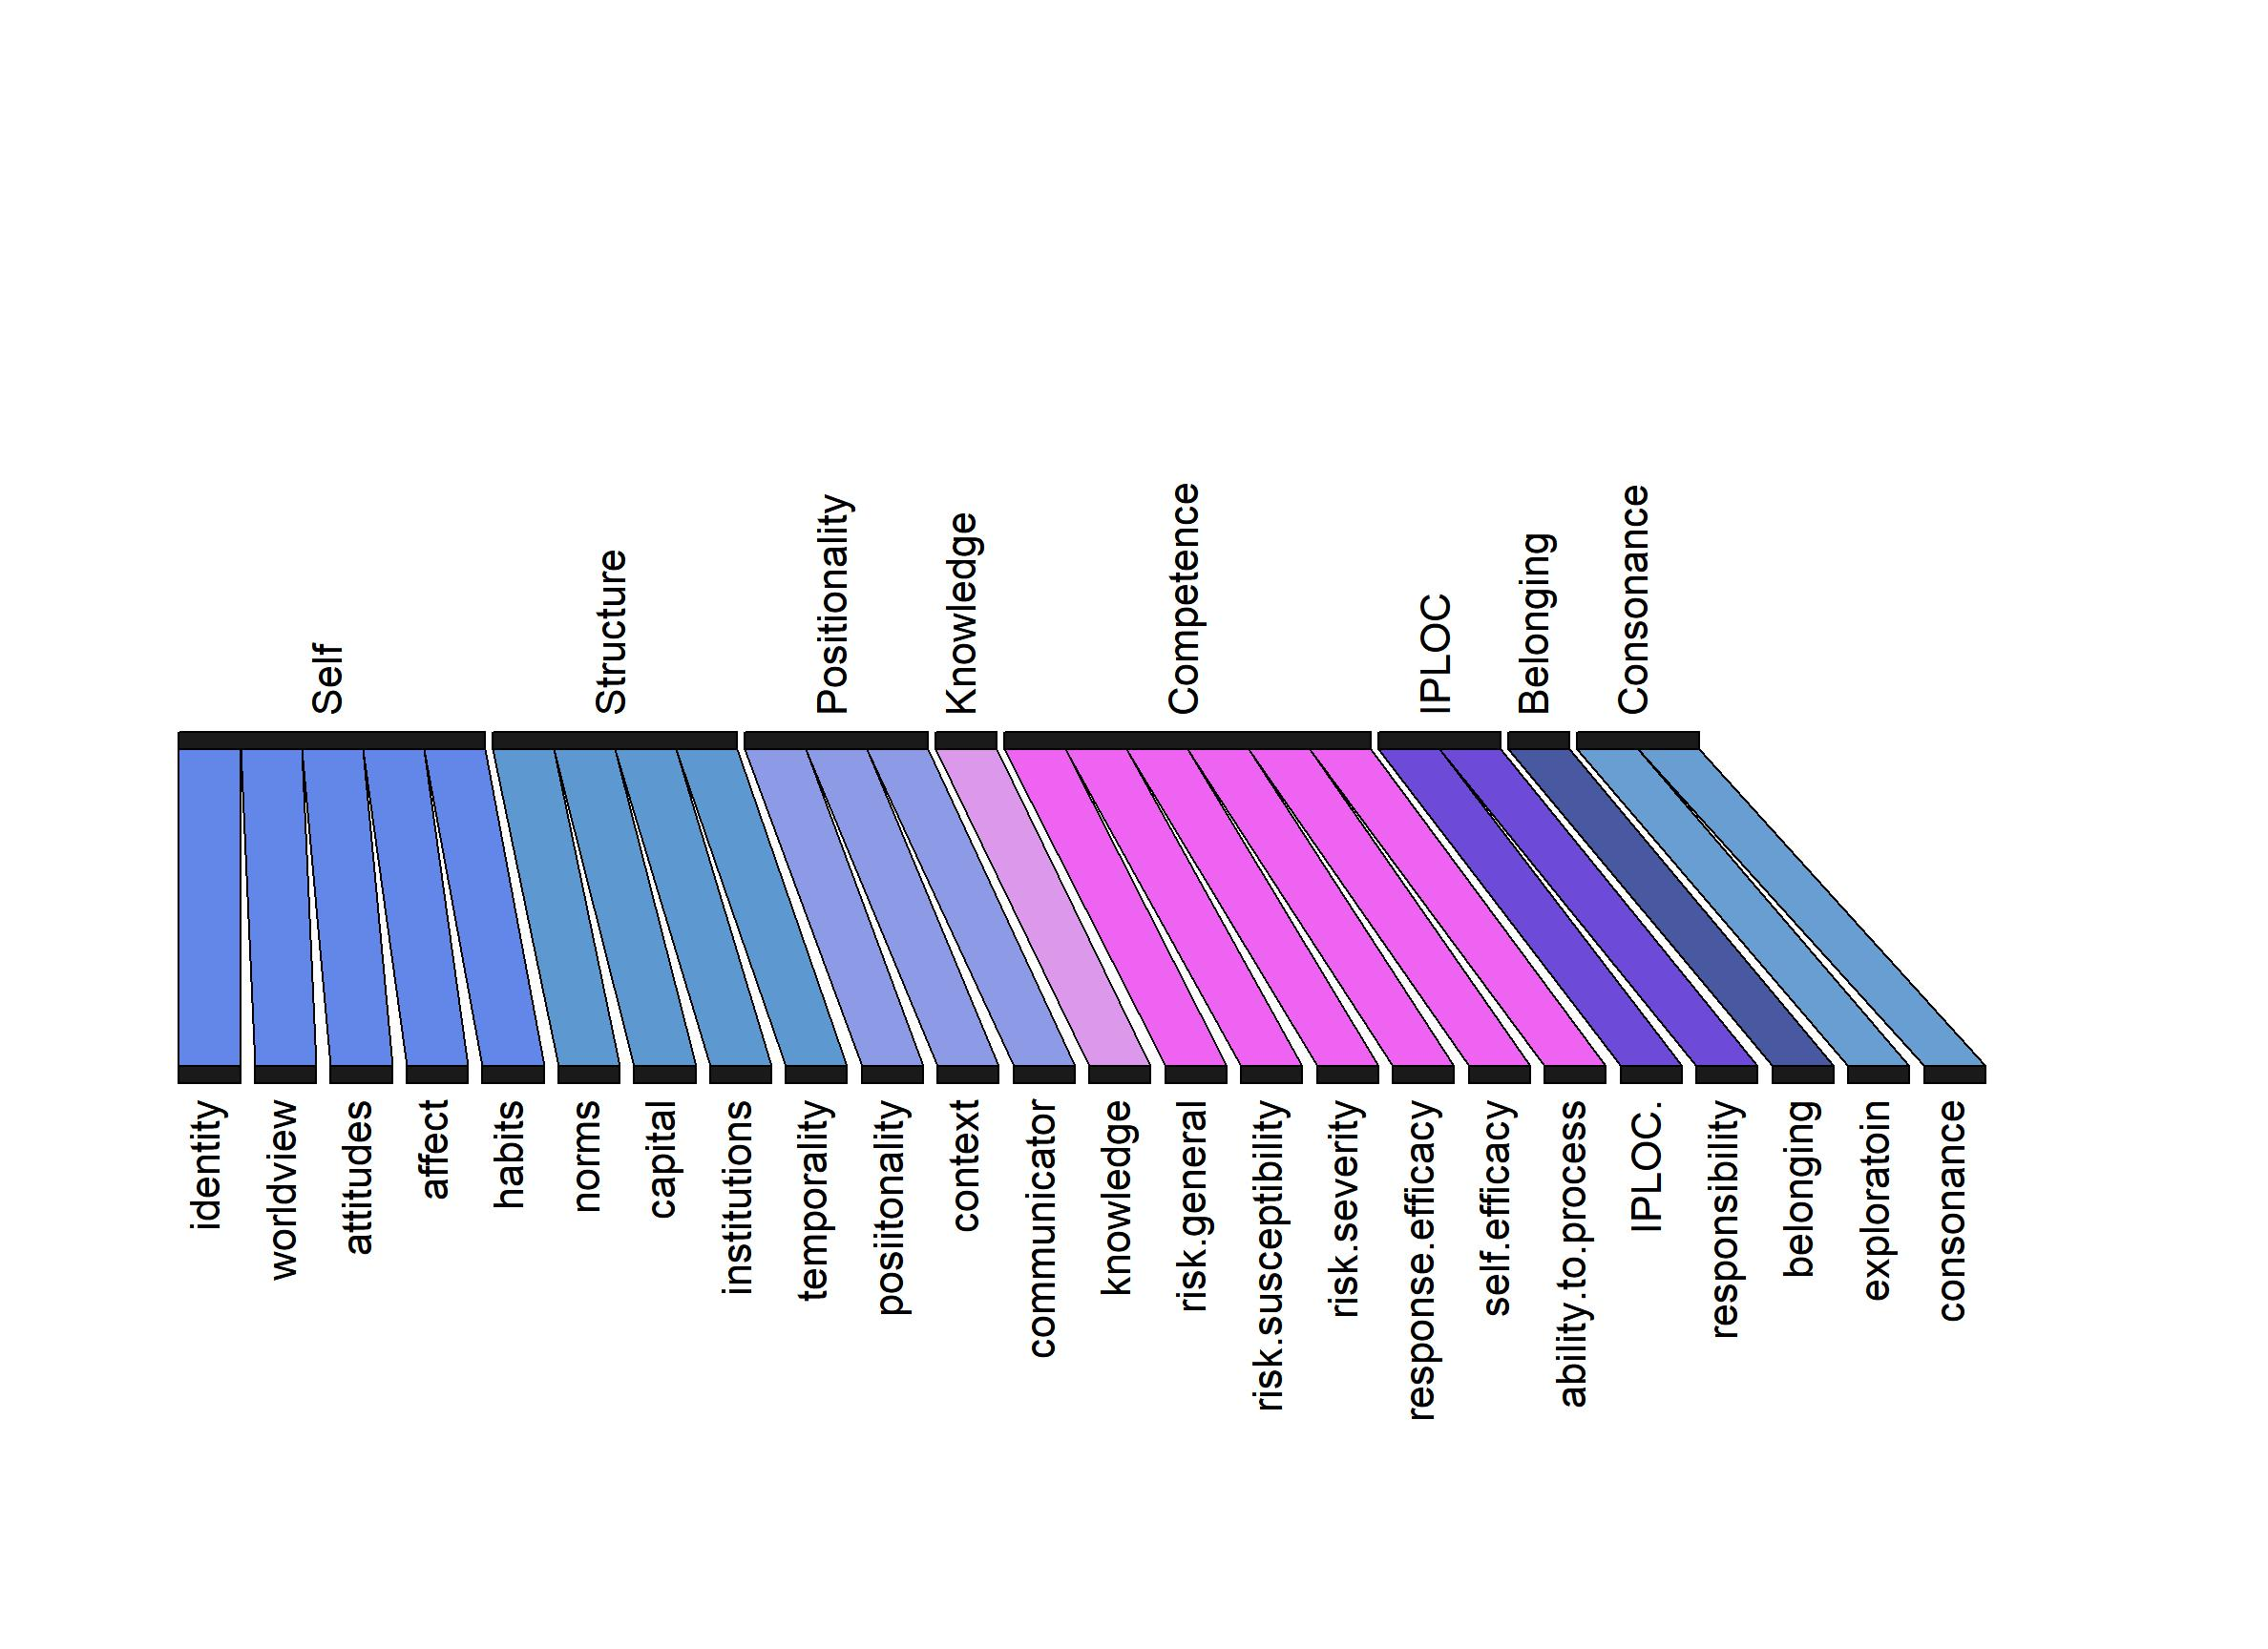
\includegraphics[width=1 \textwidth,trim=0cm 0cm 0cm 0cm, angle=270, scale=1.3, origin=c,clip=true]{unif}}
 	%x x x lower right 
 	\caption{\textit{Categorizing the 24 determinants of human action into 9 generalized factors}}
 		\label{fig:unif}
 \end{figure}

 Figure \ref{fig:unif} shows this condensation. The eight generalized determinants express the core aspects of the 54 \textit{Human Action Theories}. \textbf{Knowledge} represents the organization and gathering of information; \textbf{Positionality} represents the current situation, power dynamic, and context; \textbf{Self} contains subjective attributes, including identity, values, affect etc. \textbf{Structure} contains culture, norms, physical capital, and societal prescriptions. These four factors encode the state of the world and the humans of interest. The second four determinants dictate how these states of the world are navigated. \textbf{Consonance} contains needs for exploration, growth, and conquering incongruities; \textbf{Belonging} includes the need for being connected; \textbf{IPLOC (Internal Locus of Causation)} includes our need for autonomy, ownership, and responsibility; and finally \textbf{Competence} includes efficacy and its inverse, risk. Together, these eight factors constitute a \textbf{Unified Human Action Framework}. 
 
   \begin{figure}
   	\centering
   	\textbf{A unified human action framework}\par \medskip
   	
   	\fbox{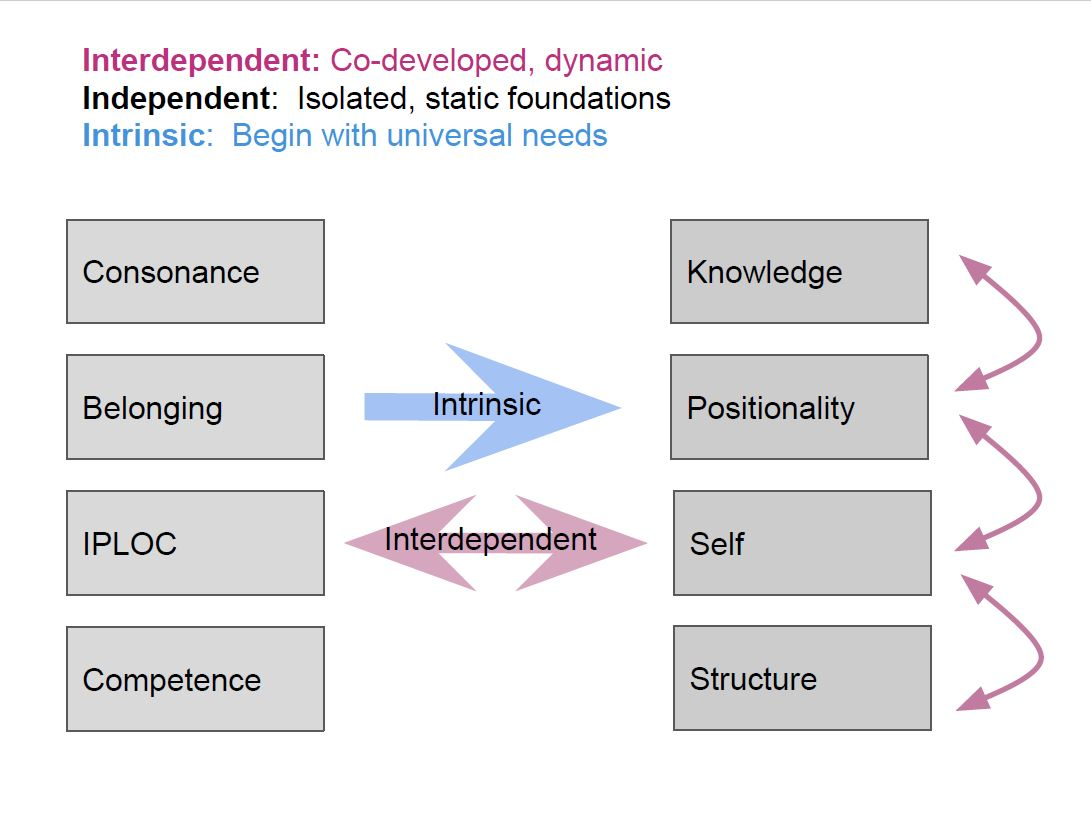
\includegraphics[width=1 \textwidth,trim=0cm 0cm 0cm 0cm, angle=0, scale=1, origin=c,clip=true]{unifdiag}}
   	%x x x lower right 
   	\caption{\textit{A diagram displaying the unified theory of human action, and the variations under different metatheories. Needs are shown on the left, and others on the right. In the Interdependent metatheory, all factors are co-developed and dependent on all the other factors. Each factor is mutable, and theorists typically look for more ultimate causes of current expressions. The independent metatheory takes the world as it is, assuming that each factor is more constrained and not co-developed by others. In the intrinsic metatheory, the factors on the left take primacy, and are universal and taken as-is. They explain how people navigate the world as explained by the factors on the right.}}
   	\label{fig:unifidag}
   \end{figure}
   
 However, as noted earlier, aggregating factors from different metatheories is not always advisable. To overcome this, my \textit{Unified Human Action Framework (UHAF)} is metatheory-explicit. Figure \ref{fig:unifidag} shows the eight determinants and how they are assumed to interact for each metatheory. In \textit{Interdependent Metatheory}, all factors are co-developed and dependent on all the other factors, and the need factors are simply emergent from the `self'. Each factor is mutable, and theorists typically look for more ultimate causes of current expressions. The \textit{Independent Metatheory} takes the world as it is, assuming that each factor is more constrained and not co-developed by others. In the \textit{Intrinsic Metatheory}, the second group of factors has primacy, are universal, and taken as-is. They explain how people navigate the world.  Robust to different metatheories, this framework represents the multidisciplinary of the \textit{Human Action Theories} it builds upon.  
  

 \begin{figure}
 	\centering
 	\textbf{Theories and their generalized attributes}\par \medskip

 	\fbox{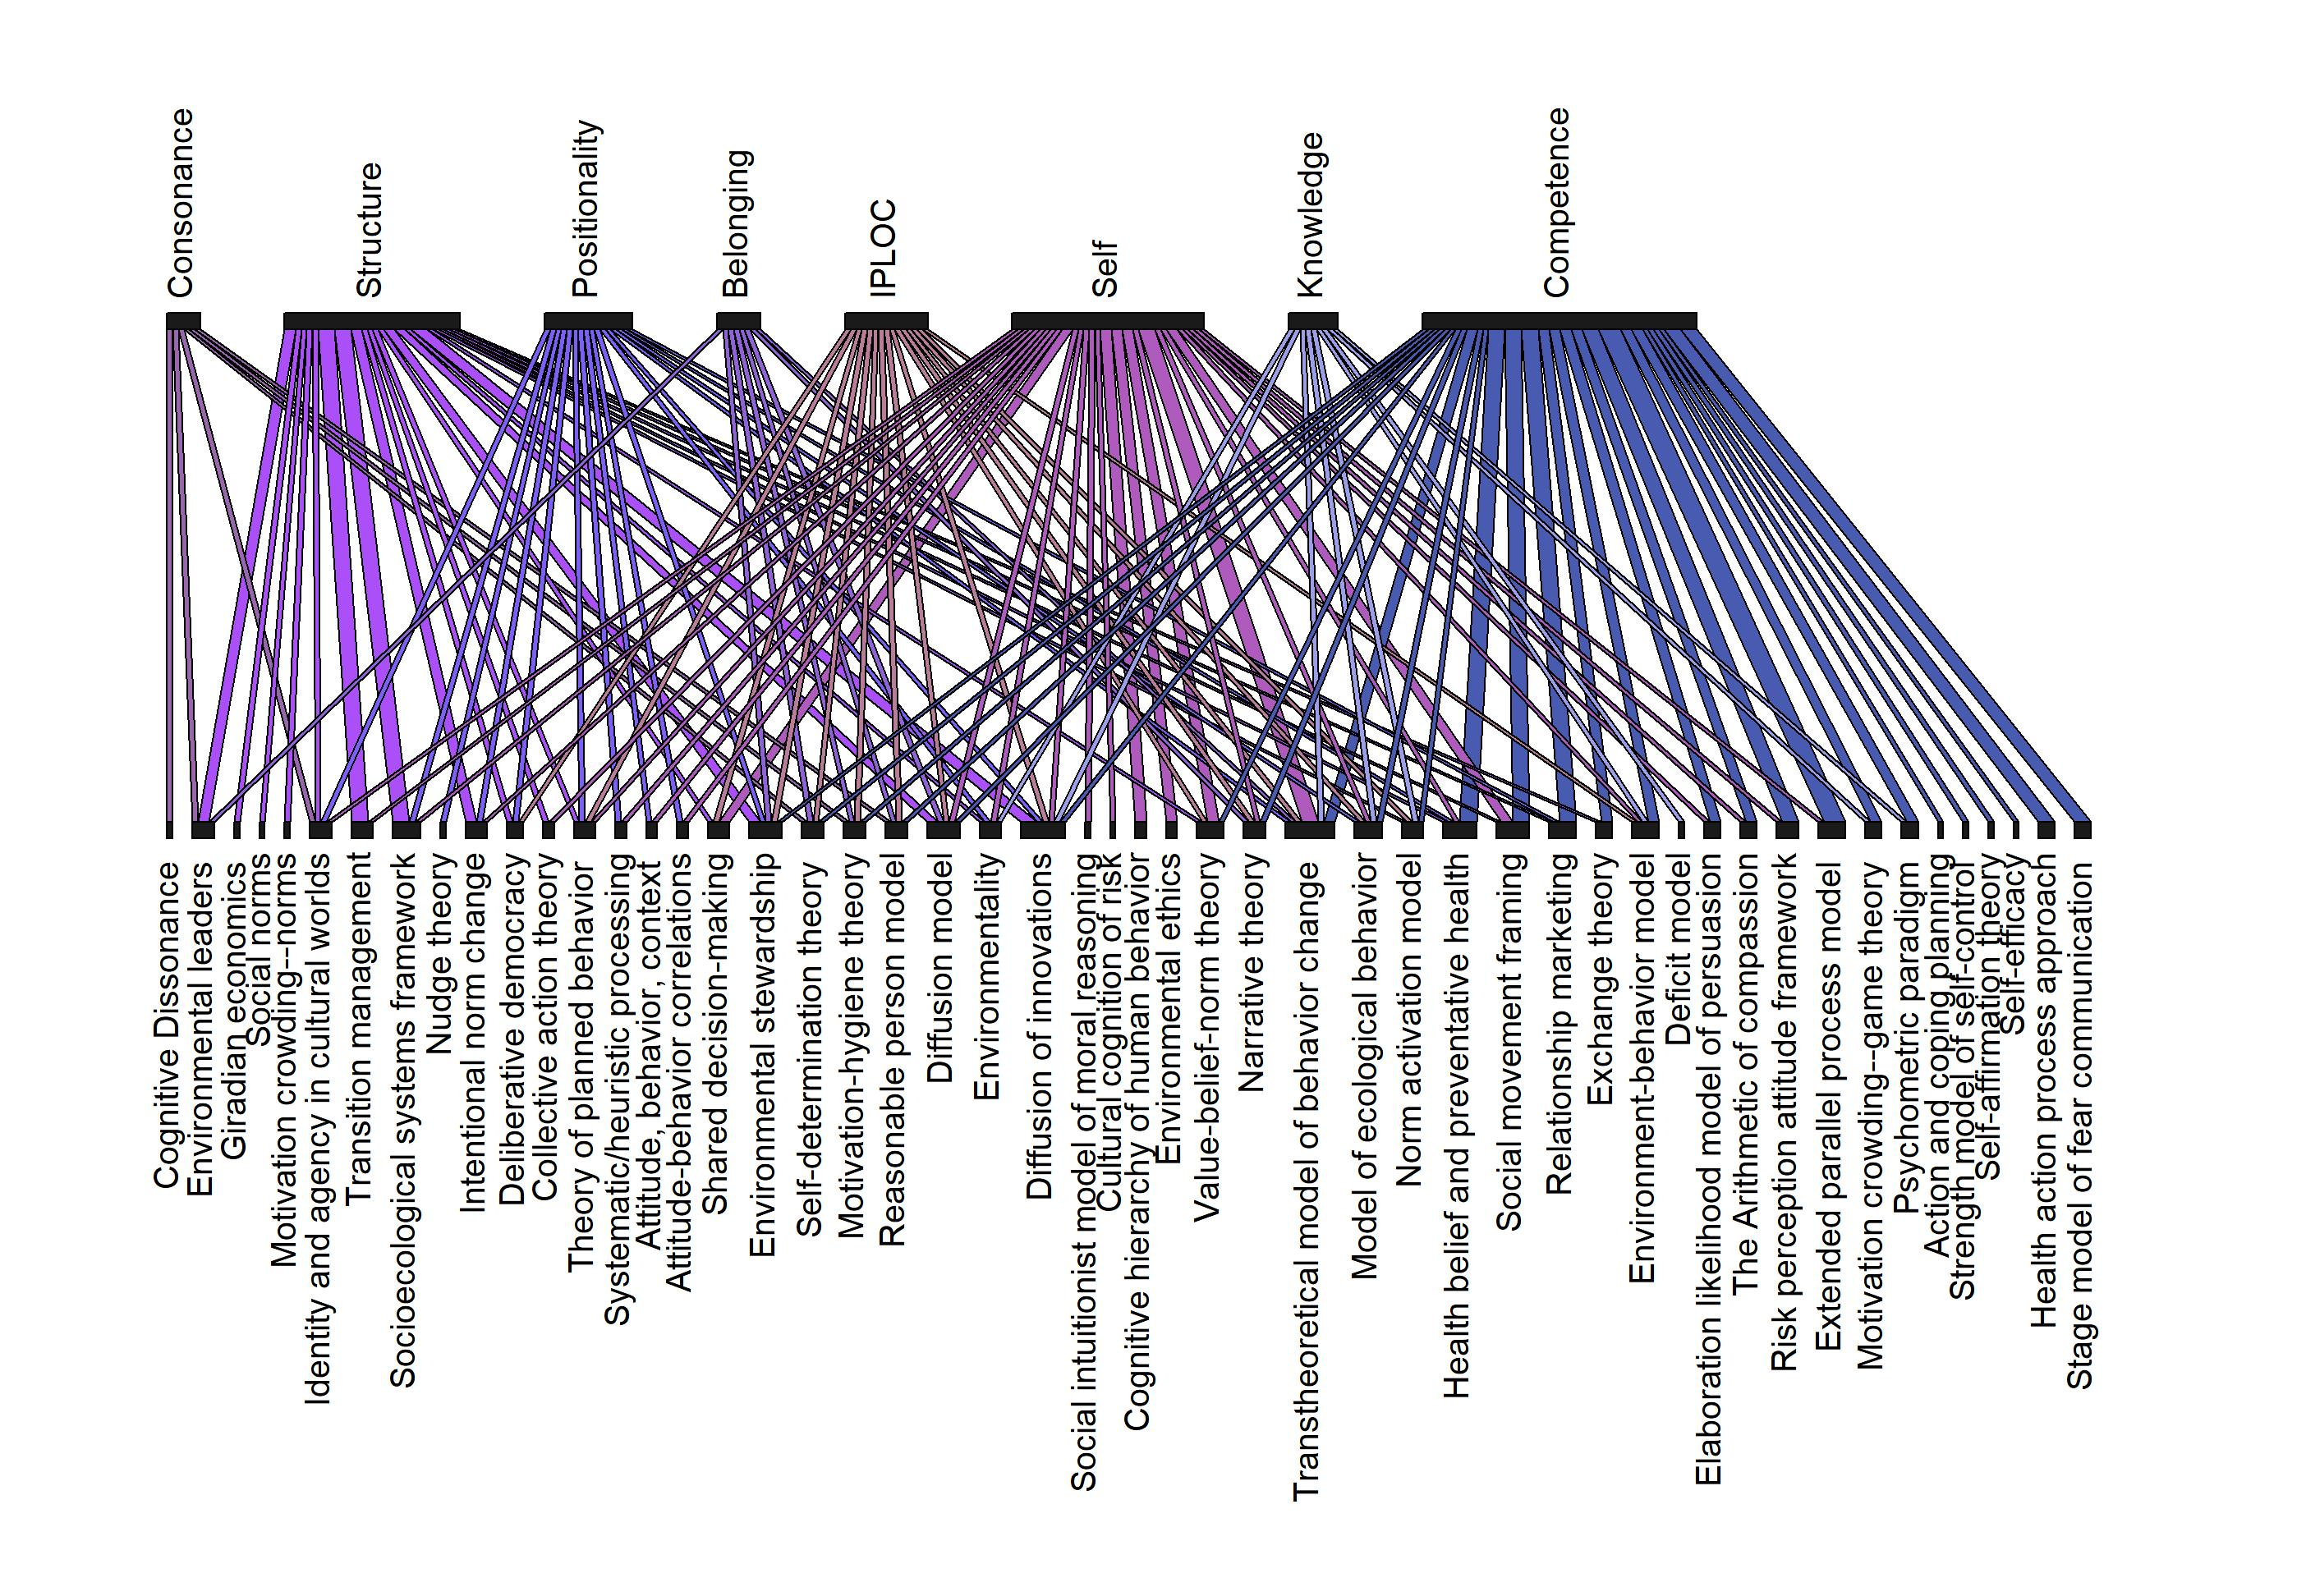
\includegraphics[width=1 \textwidth,trim=0cm 0cm 2cm 0cm, angle=270, scale=1.3, origin=c,clip=true]{unifact}}
 	%x x x lower right 
 	\caption{\textit{Different Human Action Theories utilize different sets of the nine generalized determinants}}
 	 	\label{fig:unifact}
 \end{figure}
 
  Applying this new framework back to my aggregated \textit{Human Action Theories}, Figure \ref{fig:unifact} shows that these eight determinants are broadly relevant, but many theories only include a few. This suggests that many theories may ignore important determinants. There is much room for generalizing, complementing, and identifying context specificities. For example, the stage model of fear communication does not include positionality or belonging. Would people respond differently to fear appeals if they were powerful vs. weak? If they had a close relationship with their doctor, would they be more likely to feel a sense of belongingness, and thus more likely to be motivated to take bold action to minimize the fear? This association between theories and generalized determinants highlights the narrowness of many theories, and invites many new and exciting questions.  
 
 
Organizing and unifying social science theories of human action is a seemingly insurmountable task, and one that some recommended against: ``what shapes pro-environmental behavior is such a complex one that it cannot be visualized in one single framework or diagram" \parencite[][p. 248]{Kollmuss2002}. I have attempted to do just that (see Figures \ref{fig:unifact} and \ref{fig:unifidag}). 
Perhaps these impossible endeavors are those most needing investment. \textcite{Haslam2001} suggests that scholars have been focusing too much on minimizing certain types of uncertainty, leading to conservative research that answers uninteresting questions very precisely. Instead, it is uncertainty \textit{creating} investigations that lead to scientific revolutions. Research that increases epistemological uncertainty instead of minimizing ontological uncertainty may have the biggest impact \parencite{Haslam2001}. Although these investigations are often inexact and hand-wavy, they may put focus on the new and exciting path. 

In the field of environmental science, one good example of this type of research is \textcite{Costanza1997}. This paper asked a question that was impossible to answer with very much statistical certainty: What is the value of Earth's ecosystem service? Their analysis made many gross assumptions, and their result had huge statistical uncertainty. Yet, in spite of these approximations, the paper jump-started the study of ecosystem services, revolutionizing the way we think about our reliance on natural capital.  In a similar, though likely less grandiose vein, I hope that this current paper will refocus the way we think about why people do what they do. 

Like Constanza et al. (1997), I make many generalizations and shortcuts, but I hope that like that paper, my synthesis will kindle a new appreciation for the benefits of looking beyond a particular discipline. I hope that it spurs more research into a \textbf{Unified Theory of Human Action} to the benefit of scholars, practitioners, and the planet. 
\bigskip
\bigskip
\bigskip

\printbibliography
\end{document}


%Like environmentality \parencite{Agrawal2005}, \textcite{Holland1998} suggests that the self results from a codevelopment of the person, culture, and position. The person is the sbujectivity of environmentality, while the position is the politics/knowledge, and culture is made up of institutions and knowledge. 
%
%
%From a cultualist perspective,  "The job of the anthropologist was to find the culture"\parencite{Holland1998}[p.15]
%\par \textcite{Bourdieu1977} sees culturalist interpretations as unreasonable -- life is too complex and dynamic to for decisions to be reducible to rules. Rather than rules, associations are supreme. Associations between actions/movements, figures/categories, and environments/contexts. And then it seems as though he argues that qualities (values?) like "honor" are bestowed upon a figured world (how does a figured world compare to an association?)

%Subjectivities: "figured worlds and their situated realizations" \parencite{Holland1998}[p. 286]. We are made by our actions (sophistory school; Holland1998)

%Ability to process subsumes the prominence of a stimuli, e.g., how simple it is , and how easy it is to comprehend the problem (psychic numbing) (Arithmetic of compassion ). Also covers 'experiential commensurability' of how similar someone's experiences are to the frame being profered \parencite{Benford2000}

%
%
%As per the Interdependent metatheory, these dterminants cannot be viewed alone. There is a tension between cultural logic (cultualist -- situation-transcending, product of history ) and subject position (constructavist -- situational, instrumental): "The culturalist speaker seeks to conduct herself so as to do right by a preconstituted, culturally given, and moral world. The constructivist speaker responds instead to the social claims implied by the utterance, making a sustaining the claims that the particular situation allows." 
%
%
%Combining bits from the culturalist and constructivist worldviews, \textcite{Holland1998} attempts  to "see both culture and subject position at the same time" (pp. 16-7). 

